\documentclass[a4paper,fleqn]{cas-dc}
\hypersetup{hypertexnames=false}
\usepackage[sort,numbers]{natbib}
\usepackage{amsmath}
\usepackage{amssymb}
\usepackage{amsthm}
\usepackage{algorithm}
\usepackage[commentColor=black,beginComment=//~,endComment={},beginLComment=//~,endLComment={},italicComments=false]{algpseudocodex}
\tikzset{algpxIndentLine/.style={draw=black}}
\algrenewcommand{\alglinenumber}[1]{\bfseries\footnotesize #1}
\algrenewcommand{\textproc}{}
\algrenewcommand{\algorithmicrequire}{\textbf{Input:}}
\algrenewcommand{\algorithmicensure}{\textbf{Output:}}
\newtheorem{proposition}{Proposition}
\usepackage[caption=false,font=footnotesize]{subfig}
\captionsetup[subfloat]{subrefformat=simple,labelformat=simple}
\renewcommand{\thesubfigure}{(\alph{subfigure})}
\usepackage{tabularray}
\usepackage[nameinlink]{cleveref}
\crefname{figure}{\figurename}{\figurename s}
\crefname{table}{\tablename}{\tablename s}
\crefname{equation}{}{}
\crefname{section}{Section}{Section}
\crefname{subsection}{Section}{Section}
\crefname{subsubsection}{Section}{Section}
\crefname{algorithm}{Algorithm}{Algorithms}
\crefname{proposition}{Proposition}{Propositions}
\setcounter{totalnumber}{9}
\setcounter{topnumber}{9}
\setcounter{bottomnumber}{9}
\setcounter{dbltopnumber}{9}
\renewcommand{\topfraction}{.90}
\renewcommand{\dbltopfraction}{.90}
\renewcommand{\bottomfraction}{.05}
\renewcommand{\textfraction}{.1}
\renewcommand{\floatpagefraction}{.90}
\renewcommand{\dblfloatpagefraction}{.90}
\begin{document}
\shorttitle{FedRAS}
\title[mode=title]{FedRAS: Rank Scheduling by Delivery Probability for Federated LoRA in Mobile Edge Networks}
\tnotemark[1]
\tnotetext[1]{This work was supported in part by the National Key Research and Development Program of China (No.\ 2024YFB2907201, No.\ 2024YFB2907202).}
\shortauthors{Ma et~al.}
\author[1,2,3]{Wenyu Ma}[orcid=0009-0003-9891-8062]
\ead{mwy_ndsc@163.com}
\author[1,2,3]{Xinlei Liu}[orcid=0000-0001-6586-4457]
\ead{liuxl@stu.ouc.edu.cn}\cormark[1]
\author[1,2,3]{Tao Hu}[orcid=0000-0001-7641-5622]
\ead{hutaondsc@163.com}
\cortext[cor1]{Corresponding author.}
\affiliation[1]{organization={Information Engineering University},
city={Zhengzhou},
country={China}}
\affiliation[2]{organization={Key Laboratory of Cyberspace Endogenous Safety \& Security of Henan Province},
city={Zhengzhou},
country={China}}
\affiliation[3]{organization={Key Laboratory of Cyberspace Security, Ministry of Education of China},
city={Zhengzhou},
country={China}}
\begin{abstract}
Mobile-edge federated learning (FL) lets smartphones, vehicles, and unmanned aerial vehicles (UAVs) train models collaboratively without sharing local data, a common mobile-network workload. But full-model updates frequently miss round deadlines on degraded uplinks, and once none arrives on time, the server has nothing to aggregate and learning stops. Federated low-rank adaptation (LoRA) compresses the payload by replacing full-model updates with low-rank factors, and smaller payloads arrive on time more easily. But the payload still grows with the rank, the width of the factor pair: wider factors express more change but upload more bytes, and on a deadline-constrained link the delivery probability is lower. We propose FedRAS (federated rank-adaptive scheduling), which treats the rank as a schedulable network resource and decides jointly, under a byte budget and a participation cap, who participates and at what rank, so the update size is set by the link rather than the training side. FedRAS runs a closed round loop whose three modules score every client--rank pair, solve the assignment exactly under the byte budget, and merge heterogeneous-rank updates exactly with frozen factors. Under deadline stress, FedRAS delivers the most update mass: 22\% more timely updates at 23\% fewer bytes than fixed rank 16, 42\% more than fixed rank 4, at statistically equivalent accuracy, while full-model updates deliver nothing. When the backbone is weak, these updates convert into accuracy, up to 1.3 percentage points over link-oblivious schedules. At 500 clients, once the budget binds, exact scheduling beats greedy at sub-second cost.
\end{abstract}
\begin{keywords}
Federated LoRA \sep Mobile edge computing \sep Rank selection \sep Deadline scheduling \sep Wireless federated learning
\end{keywords}
\maketitle
\section{Introduction}
\label{sec:intro}
Mobile edge networks increasingly host federated learning (FL) workloads. The participating devices include smartphones, vehicles, unmanned aerial vehicles (UAVs), and satellite-connected devices \cite{mcmahan2017fedavg,kairouz2021advances}, spanning Internet of Things (IoT) deployments \cite{nguyen2021iotfl} and space--air--ground integrated network (SAGIN) systems \cite{liu2018sagin,mahboob2024ntn}. Such systems train a model with the data never leaving the devices, but their links differ across devices and change with mobility, and the uplink is often the bottleneck of the whole system.
\par
Federated training proceeds in rounds: the server broadcasts the current model, each client trains on its local data and uploads its update before a round deadline, and the server aggregates whatever arrives on time. Full-model updates---each carrying the change of every weight in the model---saturate wireless capacity and drain device energy \cite{hamdi2022ehfl}, and once links degrade during handover or outage, they miss the round deadline all the more \cite{razmi2022ground,tang2023flsagin,qin2024dfrl,ribero2023intermittent}. Deadline-enforcing systems do not wait: clients that cannot finish are dropped outright for that round \cite{nishio2019fedcs}, with no buffering and no retransmission. Once the deadline tightens to the point that no full-model update completes on time, the round aggregates nothing at all: the broadcast model becomes the only model, and federated learning does not slow down---it stops.
\par
Federated low-rank adaptation (LoRA) therefore becomes a useful technique, because each adapted layer transmits only two low-rank factors instead of the full weight delta \cite{hu2022lora,babakniya2023slora,zhang2024fedit}. But the payload still grows with the rank, and the rank is the width of this factor pair: the larger the rank, the more change the model can learn and the lower the delivery probability.
\par
Existing federated LoRA systems treat the rank as a hyperparameter---fixed across the fleet \cite{sun2024ffalora,zhang2023fedpetuning}, varied across clients \cite{cho2024hetlora,fan2025helora}, adapted across rounds \cite{wu2026fedara,yang2024safedlora}, or personalized through model-heterogeneous and dual-adapter designs \cite{yi2026pfedlora,yang2024feddpa}. The channel-aware line of work does exploit the link state, but its optimization objective is expected latency, not the delivery probability of a specific payload within the deadline. The rank that can be delivered moves with the link---across clients, rounds, and deployment stages---so any rank fixed offline is wrong somewhere: a small fixed rank is delivered but learns too little, a large fixed rank spends bytes on uploads that never arrive, and a training-signal schedule cannot see the link at all.
\par
Each round must therefore decide jointly, under a total byte budget and a participation cap, who participates and at what rank. Three questions follow. How should the delivery probability depend on the rank and the observable link state? How should the client--rank assignment be solved under budget and participation constraints? How should the gains of scheduling in a real trainer be measured, and when do they convert into test accuracy? We invent FedRAS (federated rank-adaptive scheduling). Our contributions are threefold.
\begin{itemize}
\item Based on the trade-off between adaptation capacity and delivery probability---the larger the rank, the more change the model can learn and the lower the delivery probability---we design, to our knowledge, the first scheduling framework that treats the LoRA rank as a schedulable network resource and name it FedRAS. FedRAS runs a closed round loop with three modules, setting the rank from the per-round delivery state of the link rather than from training signals or expected latency. Action Construction (AC) scores every client--rank pair by its delivery probability and its adaptation capacity, with payloads priced at real serialized sizes. The GridDP assignment (GDP) decides admission and rank jointly under the byte budget and the participation cap, solving the assignment exactly on a byte grid. Masked Aggregation (MA) merges heterogeneous-rank updates exactly by frozen-factor averaging.
\item Based on the multiple-choice-knapsack structure of the joint assignment, we prove that GDP solves it exactly on a byte grid (\cref{prop:dp}); that under a budget-feasibility condition the closed-form per-client rule $r_i^\star=\bar R_i^t\tau/(16c)$ is already optimal, enabling a zero-cost switch (\cref{prop:cohort}); and that frozen-factor aggregation merges heterogeneous-rank updates exactly (\cref{prop:agg}).
\item On CIFAR-10, CIFAR-100, and MNIST, using a real 20-client federated LoRA trainer and a 500-client scheduler simulation, we demonstrate the superiority of FedRAS: under deadline stress, it delivers the most update mass of the evaluated policies---22\% more timely updates at 23\% fewer bytes than fixed rank 16, and 42\% more update mass than fixed rank 4---at statistically equivalent accuracy, while full-model updates deliver nothing; a backbone-quality sweep locates when preserved capacity converts into accuracy, up to 1.3 percentage points over link-oblivious schedules; and whenever the budget binds, exact scheduling beats greedy at sub-second cost.
\end{itemize}
\section{Related Work}
\label{sec:related}
\subsection{Federated LoRA: An Evolution Toward Adaptive Ranks}
\label{sec:rwlora}
LoRA replaces the full weight delta with two low-rank factors, $\Delta W=BA$, beside a frozen backbone \cite{hu2022lora}, and was ported to federated learning by sparse-update and instruction-tuning studies \cite{babakniya2023slora,zhang2024fedit}; early evaluations confirmed that parameter-efficient tuning survives the federated setting \cite{zhang2023fedpetuning}. In federated LoRA the rank follows whatever information it is set from; we call that information the rank signal, and prior work reads four kinds of it.
\par
The first kind of rank signal is an offline choice, the same for the whole fleet: the rank is a fixed hyperparameter, so the payload never responds to run-time state.
\par
The second kind of rank signal is device capability or training-side statistics. HetLoRA prunes ranks per client and repairs the average with sparsity weights \cite{cho2024hetlora}, FLoRA stacks factors to a common width \cite{wang2024flora}, HeLoRA aligns them through padded context \cite{fan2025helora}, FedARA allocates ranks by singular value decomposition (SVD) of the aggregated update \cite{wu2026fedara}, and a recent refinement aligns heterogeneous ranks at negligible overhead \cite{byun2025fedlora}. The rank now responds to the device and to training, yet not to whether this round's link can actually deliver the payload---and none of these systems prices that cost.
\par
The third kind of rank signal is training progress. SA-FedLoRA schedules the rank over rounds by training progress \cite{yang2024safedlora}, FedSA-LoRA couples it with asymmetric factor aggregation \cite{guo2025fedsalora}, and dual-adapter or model-heterogeneous designs personalize the adapter itself \cite{yi2026pfedlora,yang2024feddpa}. Whatever the refinement, the signal remains training progress, parameter importance, or device capability; the state of the lossy, deadline-constrained link never enters the decision.
\par
The fourth kind of rank signal, the channel itself, is the one closest to FedRAS. ROBA jointly optimizes per-client rank and bandwidth allocation under time-varying channels, with communication and computation latency in the objective \cite{zou2025roba}. TSFA selects the rank offline from statistical channel information and adapts sparsification and bandwidth online under delay constraints \cite{kim2025tsfa}. Adaptive federated LoRA couples sketching ratios with client sampling probabilities under bandwidth constraints to minimize wall-clock convergence time \cite{hou2025aflora}. These systems do read the link, but they optimize expected latency or convergence time and treat delivery as assured once resources are granted; none prices the delivery probability of the specific payload within the round deadline.
\par
Another line of work is concerned with how to aggregate, and FFA-LoRA is its representative. LoRA has two factors, and training usually updates both. Updating both, however, creates a problem: the same update can be written as different factor combinations, so when the server holds the factors uploaded by many clients, averaging them directly is meaningless---the factors do not align. FFA-LoRA freezes one of the two factors at initialization, originally for training stability in privacy-preserving fine-tuning \cite{sun2024ffalora}; its setting assumes the same rank for every client, so it never faces the question of merging different ranks. FedRAS keeps the frozen factor but applies it to the heterogeneous ranks the scheduler chooses: factor slices uploaded at different ranks land on the same coordinates, and averaging, column by column, whatever arrives on time is exact averaging of the active update slices (\cref{prop:agg})---no alignment step, and none of the misalignment of training both factors. The scheduler can therefore assign different ranks to different clients while the aggregation layer still merges them exactly, and scheduling and aggregation meet. HetLoRA-style sparsity weighting can be read as a weighted variant of this average, but it normalizes with one common denominator, so high-rank slices are diluted by low-rank clients; FedRAS normalizes each column by the clients that actually cover it, keeps the high-rank information intact, and this is exactly where the exactness of its aggregation comes from.
\subsection{Communication-Efficient Federated Learning}
FedRAS and compression do not solve the same problem. Compression decides how to transmit a given object in fewer bits; FedRAS decides how large an object to transmit over a given link. Sparsification \cite{lin2018deep}, quantization \cite{liu2023adaptivequant,reisizadeh2020fedpaq}, quantized compressed sensing \cite{oh2023fedqcs,oh2024fedvqcs}, and over-the-air aggregation \cite{kim2023beamforming} do compress the payload, and codec adaptation tracks channel state. But no codec decides the size of the object it encodes, and compression cannot recover a deadline that an already-oversized payload is destined to miss. FedRAS selects the rank before transmission, swapping a payload destined to miss this round for a smaller one that arrives on time, and so preserves the update mass. Compression, in turn, can only shrink the payload after it is chosen; it cannot change whether that payload arrives. Compression acts on the payload FedRAS has chosen: the two work at different stages, compose freely, and do not replace each other. Compression and scheduling can therefore be used together---one decides how large to transmit, the other how to transmit it in fewer bits.
\subsection{Client Selection and Deadline-Aware Scheduling}
\label{sec:rwselect}
Client selection decides who participates---but in all of this work the payload size is an input, never a decision. Oort ranks candidates by a utility that couples data value with system efficiency \cite{oort2021oort}, FedCS admits clients under explicit resource constraints \cite{nishio2019fedcs}, and TiFL bounds stragglers through latency tiers \cite{chai2020tifl}; further designs target heterogeneity, cost, and freshness \cite{chen2024clientselection,dong2024aoi,luo2021costeffective}. Deadline- and reliability-aware schedulers extend admission to mobile and non-terrestrial networks, from participation under handover and outage \cite{razmi2022ground,tang2023flsagin,ribero2023intermittent,han2024orchestrating} to offloading driven by federated reinforcement learning \cite{qin2024dfrl}, with LESSON admitting wireless clients at differentiated frequencies under a latency budget \cite{yu2023lesson} and FedSN coordinating training over heterogeneous low-Earth-orbit (LEO) constellations \cite{lin2025fedsn}. These systems fold the deadline into admission, but the payload remains given, so the choice is only among updates of a fixed size. Such a system has two options---transmit an oversized payload that is destined not to arrive, or skip the update entirely---because it cannot break the payload down to a size the link can carry. Once the payload itself becomes a decision, the problem changes in nature: every client carries several rank options, each with its own bytes and gains, and the choice is no longer a ranking or a threshold but the selection of a combination under the byte budget and the participation cap, in which greedy rules are not necessarily optimal (\cref{prop:dp,prop:cohort}). The advantage of FedRAS is that it merges selection and payload into one decision, using exact scheduling to decide who participates and at what rank; an update that could previously only be skipped or forced through can be shrunk to a size the link delivers on time, so more timely updates are delivered under the same budget and deadline. This is why FedRAS needs a new solver rather than a rank parameter added to an existing selector, and why an Oort-style selector can here serve only as the baseline: it cannot handle the case where each client carries several payload options.
\subsection{Research Gap and Positioning}
Across the surveyed lines, the update size is fixed by the training side: rank methods read training progress or device capability, the wireless-aware line reads the channel but prices expected latency, and selection methods schedule a payload they did not choose. None treats the LoRA rank as a schedulable network resource priced by the payload's delivery probability, and none solves admission and rank jointly under a byte budget and a deadline. FedRAS fills exactly this gap: the rank is priced at its real serialized size, conditioned on the per-round delivery state of the link, and decided jointly with admission. \cref{tab:rwcompare} positions FedRAS against the closest systems; throughout the table, the delivery-aware column is the watershed, and the table note defines it---conditioning on the per-round payload delivery probability, not merely reading the channel, which is why ROBA and TSFA remain $\times$.
\par
\par
\begin{table*}[pos=tbp]
\centering
\rmfamily
\small
\caption{Positioning against federated LoRA and client-selection systems. \checkmark{} = the property holds in the cited papers' own descriptions; $\times$ = absent or not reported. Delivery-aware means that a scheduling or adaptation decision conditions on per-round network delivery state (rate, deadline, delivery probability) rather than on training progress, device capability, or static profiling alone; the wireless-aware rank line (ROBA, TSFA, adaptive FL) reads channel state but optimizes expected latency or convergence time with delivery assumed once resources are granted, so it is not delivery-aware in this per-payload sense. Real payload means payload is accounted as transmitted bytes rather than a fixed or parameter-count proxy. Real training means model training is executed in the evaluation as reported.}
\label{tab:rwcompare}
\begin{tblr}
{
columns={co=-1},
cells={valign=m,halign=c},
columns={colsep=3pt},
rows={rowsep=2pt},
rows={ht=0pt},
stretch=0,
hline{1,Z}={wd=.08em},
hline{2}={wd=.05em},
cells={font=\fontsize{9pt}{9pt}},
row{1}={font=\bfseries\boldmath\fontsize{9pt}{9pt}},
cell{Z}{1}={font=\bfseries\boldmath\fontsize{9pt}{9pt}},
row{even[2]}={bg=gray9!35},
}
System & Var. rank & Deliv.-aware & Het.-rank agg. & Admission & Joint adm.+rank & Real payload & Real training \\
FFA-LoRA \cite{sun2024ffalora} & $\times$ & $\times$ & $\times$ & $\times$ & $\times$ & $\times$ & \checkmark \\
SLoRA \cite{babakniya2023slora} & $\times$ & $\times$ & $\times$ & $\times$ & $\times$ & $\times$ & \checkmark \\
FedDPA \cite{yang2024feddpa} & $\times$ & $\times$ & $\times$ & $\times$ & $\times$ & $\times$ & \checkmark \\
HetLoRA \cite{cho2024hetlora} & \checkmark & $\times$ & \checkmark & $\times$ & $\times$ & $\times$ & \checkmark \\
HeLoRA \cite{fan2025helora} & \checkmark & $\times$ & \checkmark & $\times$ & $\times$ & $\times$ & \checkmark \\
FedARA \cite{wu2026fedara} & \checkmark & $\times$ & \checkmark & $\times$ & $\times$ & $\times$ & \checkmark \\
SA-FedLoRA \cite{yang2024safedlora} & \checkmark & $\times$ & $\times$ & $\times$ & $\times$ & $\times$ & \checkmark \\
FedSA-LoRA \cite{guo2025fedsalora} & $\times$ & $\times$ & $\times$ & $\times$ & $\times$ & $\times$ & \checkmark \\
ROBA \cite{zou2025roba} & \checkmark & $\times$ & $\times$ & $\times$ & $\times$ & $\times$ & $\times$ \\
TSFA \cite{kim2025tsfa} & \checkmark & $\times$ & $\times$ & $\times$ & $\times$ & $\times$ & $\times$ \\
Adapt.\ FL \cite{hou2025aflora} & \checkmark & $\times$ & $\times$ & \checkmark & $\times$ & $\times$ & $\times$ \\
Oort \cite{oort2021oort} & $\times$ & $\times$ & $\times$ & \checkmark & $\times$ & $\times$ & \checkmark \\
FedCS \cite{nishio2019fedcs} & $\times$ & \checkmark & $\times$ & \checkmark & $\times$ & $\times$ & \checkmark \\
TiFL \cite{chai2020tifl} & $\times$ & $\times$ & $\times$ & \checkmark & $\times$ & $\times$ & \checkmark \\
LESSON \cite{yu2023lesson} & $\times$ & \checkmark & $\times$ & \checkmark & $\times$ & $\times$ & \checkmark \\
FedSN \cite{lin2025fedsn} & $\times$ & \checkmark & $\times$ & \checkmark & $\times$ & $\times$ & \checkmark \\
FedRAS (ours) & \checkmark & \checkmark & \checkmark & \checkmark & \checkmark & \checkmark & \checkmark \\
\end{tblr}
\end{table*}
\par
\par
\section{System Model and Threat Model}
\label{sec:model}
\par
\begin{figure*}[pos=tbp]
\centering
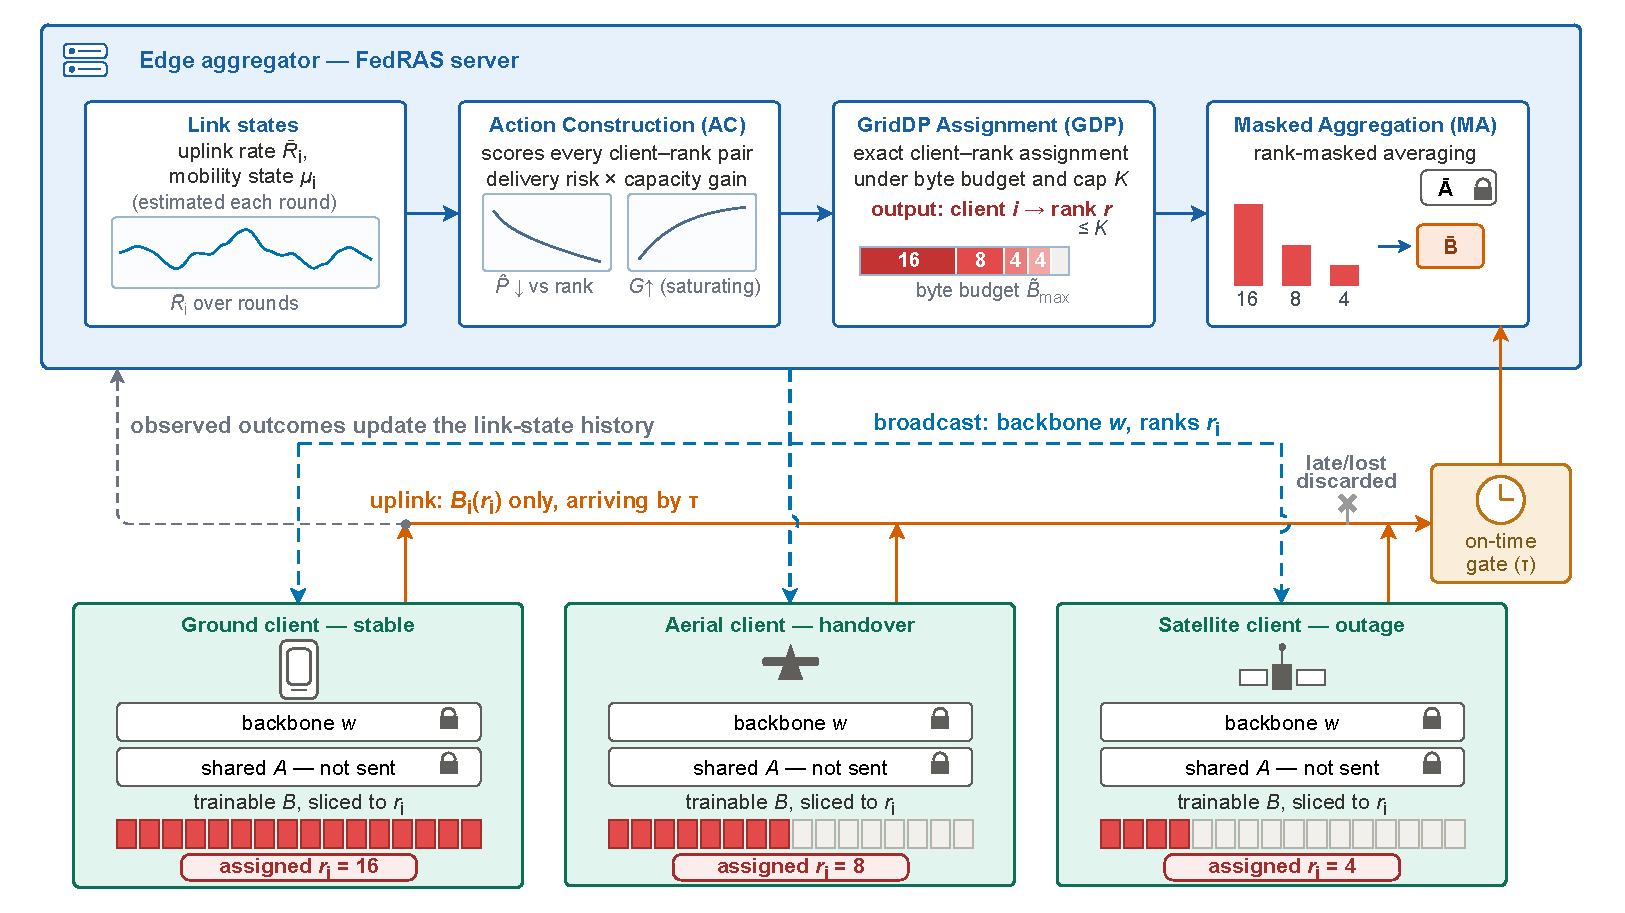
\includegraphics[width=\linewidth]{RASjiagoutu.pdf}
\caption{The FedRAS architecture. Action Construction (AC) scores every client--rank pair with the hazard model \cref{eq:hazard} and the saturating capacity \cref{eq:cap}; the GridDP assignment (GDP) computes the client--rank assignment under the byte budget and the participation cap. Updates arriving within the deadline $\tau$ pass the on-time gate and are merged by Masked Aggregation (MA) while the shared factor $A$ stays frozen; observed outcomes update the link-state history. AC, GDP, and MA correspond to \cref{alg:ac,alg:gdp,alg:ma}; the overall round is \cref{alg:fedras}.}
\label{fig:architecture}
\end{figure*}
\par
\subsection{Mobile-Edge Federated Learning Architecture and Round Protocol}
We consider a mobile edge network in which an edge aggregator serves a client set
$\mathcal{D}=\mathcal{D}_g\cup\mathcal{D}_a\cup\mathcal{D}_s$ of ground clients $\mathcal{D}_g$, aerial and UAV clients $\mathcal{D}_a$, and satellite-connected clients $\mathcal{D}_s$. Ground links are comparatively stable, aerial links face frequent handover, and satellite links suffer long propagation delay, intermittent visibility, and outages \cite{mahboob2024ntn,razmi2022ground}. The aggregator holds the global model, schedules every round, and aggregates the timely updates. This network is also the running example followed throughout the paper. The participants are the client fleet, one aggregator per region, and a passive uplink eavesdropper. The service flow repeats each round. The server, which has centrally pretrained the backbone on its own corpus, broadcasts the frozen backbone and the shared factor and attaches the round schedule. Scheduled clients fine-tune their factor slices on private local data, which never leaves the devices, and upload before the deadline. The server returns the masked aggregate of whatever arrived on time. Disclosure is controlled by the aggregator alone, through the admission and rank decisions, since a client transmits exactly the coordinates of its assigned rank. What the eavesdropper can reconstruct from an interception is therefore the induced update of that rank, the weight change its transmitted coordinates produce, and nothing beyond it. Whether the transmitted coordinates reveal training information is a question FedRAS does not claim to answer, and smaller ranks strictly reduce the exposed bytes and coordinates.
\par
Let $w^t$ denote the frozen backbone broadcast at round $t$. Client $i$ trains LoRA factors $A_{i,\ell}$ and $B_{i,\ell}$ for the adapted layers $\ell\in\mathcal L$, with effective weight change $\Delta W_{i,\ell}=B_{i,\ell}A_{i,\ell}$. A rank $r$ update uses the first $r$ columns of $B_{i,\ell}$ and the matching rows of the shared $A$. \cref{fig:architecture} shows the resulting architecture. In every round, the aggregator estimates the link states, scores the client--rank actions with Action Construction (AC), and solves the assignment with the GridDP assignment (GDP); the admitted clients train locally with their factors sliced to the assigned rank, so only the first $r$ coordinates receive gradient updates, and upload before the deadline $\tau$; the aggregator then merges the timely updates with Masked Aggregation (MA) and updates its link-state history from the observed outcomes. Late or lost updates are discarded, because stale updates harm convergence stability in deadline-critical federated learning. The experiments evaluate both a homogeneous link profile and a grouped ground--aerial--satellite profile with distinct rate and mobility laws.
\par
\subsection{Threat Model}
\label{sec:threat}
\textbf{Adversary and capabilities.} The external adversary is a passive eavesdropper on the wireless uplink: it observes the $B$ factors a client transmits, the public frozen factor $A$, and the round schedule, and nothing else, it cannot modify or drop messages (integrity and availability belong to the link model), cannot observe local data, and mounts no active attack.
\par
\textbf{Trust, assumptions, and boundary.} Clients are honest but curious, they follow the training protocol, and raw data never leaves the devices, the standing premise of federated learning on this infrastructure. The edge aggregator is trusted scheduling infrastructure: it observes link states, client--rank assignments, and delivered update factors, and runs the masked aggregation. Delivery outcomes follow the link model of the next section; clients report nothing beyond what any FL round makes observable.
\par
\textbf{Protection target.} Because $A$ is public and a rank-$r$ client transmits only its first $r$ coordinates, the object reconstructable from an intercepted transmission is the rank-$r$ induced update, and the exposed surface is its $B$-slice: strictly smaller in bytes and in exposed coordinate count than a joint-factor or full-model upload. This reduction in exposed transmission is a communication property, and it is the only security-relevant claim made here: defending the transmission content itself, together with differential-privacy accounting, secure aggregation, and Byzantine robustness, is out of scope and composes orthogonally with rank scheduling. Every method and experiment with FedRAS stays inside this boundary; no attack is mounted and no defense is evaluated.
\par
\subsection{Link, Mobility, and Timely-Delivery Model}
At decision time the scheduler receives an estimated uplink rate $\bar R_i^t$ in Mbps and a mobility state. The realized rate $R_i^t$, handover event $H_i^t\in\{0,1\}$, and packet loss indicator $J_i^t$ are not observed before transmission. For an update of $B_i^t(r)$ megabytes, the modeled delivery time is
\begin{equation}
T_i^t(r)=T_{\rm train,i}(r)+T_{\rm proc,i}(r)+\frac{8B_i^t(r)}{R_i^t}+d_i^t+H_i^t\Delta d_h.
\label{eq:delivery}
\end{equation}
Timely delivery is the event
\begin{equation}
P_{\rm on,i}^t(r)=\Pr\!\left(T_i^t(r)\le\tau,\;J_i^t=0\mid x_i^t\right).
\label{eq:pon}
\end{equation}
\par
Deriving an analytical delivery-time distribution for every term of \cref{eq:delivery} under real mobility and handover dynamics is non-trivial. Two conventions make the model operational. First, $\tau$ is the uplink delivery window that opens when local training finishes: the deadline binds the transmission, propagation, and handover terms, and every experiment interprets it this way. Second, the rank-dependence of $T_{\rm train}$ and $T_{\rm proc}$ is absorbed, as a stated approximation, into the rank-independent intensity $\mu_i^t$; for the evaluated backbones the adapters hold at most a few percent of the parameters, so the rank-dependence of local compute is second-order, and the setup reports the measured local training time. The product form assumes the loss event and the delay event are independent; at the nominal calibration the mobility factor dominates the ratio while at the stress calibrations the transmission factor does, which keeps the two effects separable in the analysis. We therefore adopt the surrogate hazard model, a closed-form failure-risk factor in the survival-analysis sense standing in for the event \cref{eq:pon},
\begin{equation}
\hat P_{\rm on,i}^t(r)=\exp\!\big(-\mu_i^t\big)\exp\!\Big(-\frac{8B_i^t(r)}{\bar R_i^t\tau}\Big).
\label{eq:hazard}
\end{equation}
The dimensionless intensity $\mu_i^t$ summarizes mobility-related failure risk, packet loss, handover effects, and unmodeled processing time. Equation \cref{eq:hazard} therefore serves as a closed-form plug-in predictor, and the sensitivity and calibration studies quantify how prediction imperfections degrade the scheduling objective.
\par
\subsection{Rank-Dependent Payload and Adaptation Capacity}
With $b$ bits per parameter and the frozen factor $A$ shared and never transmitted, a rank-$r$ client uploads only the trainable factor $B$, whose per-rank cost is the summed output dimension $D=\sum_{\ell\in\mathcal L}d_\ell$ of the adapted layers. The real serialized payload is
\begin{equation}
B_i^t(r)=\frac{b}{8}\,r\,D+B_{\rm meta},
\label{eq:size}
\end{equation}
in bytes. Rank is therefore a schedulable network resource: it scales both the adaptation capacity and the transmission time, and its per-unit payload is audited against the evaluated model. We model the useful contribution of a delivered rank-$r$ update with the saturating capacity gain
\begin{equation}
G_i^t(r)=\pi_i^t\,\sqrt{\min(r,r_{\max})/r_{\max}},
\label{eq:cap}
\end{equation}
where $\pi_i^t$ is a per-client contribution prior in the spirit of Oort-style utility \cite{oort2021oort}. The width $r_{\max}$ is the factor width provisioned at all clients. The square root encodes the diminishing returns the delivered-update norms exhibit in the trainer, with saturation at the provisioned width; that the norm is a faithful proxy for training contribution is the underlying modeling assumption, which the sensitivity analysis bounds by sweeping the exponent. Full-model FedAvg updates \cite{mcmahan2017fedavg} are accounted at their true serialized size (\cref{tab:audit}).
\subsection{Deadline-Constrained Client--Rank Scheduling Formulation}
\label{sec:problem}
Each round, the aggregator decides $a_i^t\in\{0\}\cup\mathcal R$, where $a_i^t=0$ means client $i$ does not participate and $a_i^t=r$ schedules it at rank $r$. The per-round problem is
\begin{equation}
\max_{\{a_i^t\}}\;\sum_{i\in\mathcal D}\mathbf 1\{a_i^t>0\}\,G_i^t(a_i^t)\,P_{\rm on,i}^t(a_i^t)
\label{eq:objective}
\end{equation}
\begin{equation}
\text{s.t.}\quad \sum_i B_i^t(a_i^t)\le B_{\max},\qquad \sum_i\mathbf 1\{a_i^t>0\}\le K .
\label{eq:constraints}
\end{equation}
The objective is a scheduling utility: the expected amount of useful adaptation capacity delivered on time in the round; $B_{\max}$ is the per-round byte budget and $K$ the participation cap. Increasing $r$ raises $G$ sublinearly while lowering the delivery term, so the two effects are priced in one common unit; we call the realized quantity---the update mass actually aggregated on time, measurable in the trainer from delivered update norms---the \emph{delivered adaptation capacity}, and it serves as the single learning-side currency of the evaluation. The utility is not a surrogate for test accuracy, and its relation to accuracy is established empirically rather than assumed. When the frozen backbone is already accurate, rank choice and final accuracy are equivalent within a small pre-fixed margin, which the evaluation verifies with a two one-sided tests (TOST) procedure; this invariance is not a defect of the formulation but its enabling condition, since exactly because accuracy does not depend on the rank, the rank is free to be set by the link. When the backbone is weak enough to need adaptation, the capacity this utility maximizes converts into measured accuracy: a backbone-quality sweep characterizes the conversion, and the evaluation reports tasks where federated communication buys roughly three accuracy points over the frozen backbone itself, about one point when the pretraining and deployment input distributions differ, and a collapse to the minimum rank when the capacity term is removed. The experiments therefore report accuracy and the delivered-capacity outcomes as separate metrics, and the correspondence between them is carried by the capacity term.
\section{FedRAS Design}
\label{sec:solver}
\subsection{Overview}
\cref{alg:fedras} summarizes one round and \cref{fig:architecture} places the stages. The three design questions of \cref{sec:intro} map one-to-one onto the three modules. Action Construction (AC) answers how the rank should be priced: it scores every client--rank pair with a real payload, a delivery probability, and a capacity gain, so the exchange between capacity and delivery is settled before any decision is made. The GridDP assignment (GDP) answers how admission and rank should be decided together: it solves the scored assignment exactly under the byte budget and the participation cap, with a cheap per-client rule covering the unconstrained regime. Masked Aggregation (MA) answers how heterogeneous-rank updates can be merged without error: it averages the delivered factor slices exactly toward the frozen shared factor. The design contains no training-side logic: admissions and ranks are chosen from network state alone.
\par
\begin{algorithm}[tbp]
\caption{FedRAS Round}
\label{alg:fedras}
\begin{algorithmic}[1]
\Require clients $\mathcal D$, rank set $\mathcal R$, cap $K$, budget $B_{\max}$, deadline $\tau$, link-state history $\mathcal H^{t-1}$
\Ensure assignment $a^t$; new adapter state $S^t$; updated history $\mathcal H^t$
\State Estimate per-client link states $x_i^t$ from $\mathcal H^{t-1}$
\State Score all pairs $(i,r)$: utilities $u_i(r)$ and integer costs $\widetilde B_i(r)$ (AC, \cref{alg:ac})
\State Solve the assignment $a^t$ under $K$ and $B_{\max}$ (GDP, \cref{alg:gdp}); when the all-$r_{\max}$ profile is budget-feasible, the per-client maximizer rule is already optimal (\cref{prop:cohort})
\State Broadcast the backbone $w^t$; admitted clients train locally with factors sliced to $a_i^t$ and upload before $\tau$
\State Pass uploads arriving within $\tau$ (on-time gate)
\State Aggregate timely updates with the frozen shared $A$ (MA, \cref{alg:ma})
\State Append observed outcomes (timely, late, lost) to $\mathcal H^t$
\end{algorithmic}
\end{algorithm}
\par
\subsection{Action Construction (AC)}
\label{sec:ac}
Each round the aggregator selects, for every client, one action from the discrete set $a_i^t\in\{0\}\cup\mathcal R$ of the formulation. AC builds and scores this action set (\cref{alg:ac}): the per-rank payload follows \cref{eq:size}, the hazard model \cref{eq:hazard} and the capacity gain \cref{eq:cap} give the estimated utility $u_i(r)=G_i^t(r)\hat P_{\rm on,i}^t(r)$, and a conservative discretization onto a budget grid $q$ yields the integer cost $\widetilde B_i(r)=\lceil B_i^t(r)/q\rceil$ and the integer budget cap $\widetilde B_{\max}=\lfloor B_{\max}/q\rfloor$: rounded-up costs never understate a bill and a rounded-down cap never overstates the budget, so every grid-feasible plan is feasible in true bytes. The same grid is applied to the dynamic program, the greedy baselines, and the admission checks, so that every scheduling method optimizes over the identical feasible region; under it the estimated problem becomes a multiple-choice knapsack with a participation constraint, solvable exactly by a dynamic program (DP) whose cost grows with the numeric budget (\cref{prop:dp}); the solver study reports the evaluated grid width and the induced quantization error.
\par
\begin{algorithm}[tbp]
\caption{Action Construction (AC)}
\label{alg:ac}
\begin{algorithmic}[1]
\Require clients $\mathcal D$, ranks $\mathcal R$, budget grid $q$, link states $\{x_i^t\}$
\Ensure scored action set $\{u_i(r),\,\widetilde B_i(r)\}_{i\in\mathcal D,\,r\in\mathcal R}$
\For{each client $i$ and rank $r$}
\State Payload $B_i^t(r)$ by \cref{eq:size}; integer cost $\widetilde B_i(r)\gets\lceil B_i^t(r)/q\rceil$
\State Delivery probability $\hat P_{\rm on,i}^t(r)$ by \cref{eq:hazard}; capacity $G_i^t(r)$ by \cref{eq:cap}
\State Utility $u_i(r)\gets G_i^t(r)\,\hat P_{\rm on,i}^t(r)$
\EndFor
\State \Return the scored set; pairs with $\widetilde B_i(r)>\widetilde B_{\max}$ are infeasible
\end{algorithmic}
\end{algorithm}
\par
\subsection{GridDP Assignment (GDP)}
\label{sec:gdp}
GDP solves the scored assignment exactly (\cref{alg:gdp}). Let $V_i(k,b)$ be the maximum estimated utility from the first $i$ clients with $k$ admissions and integer budget $b$. Initialize $V_0(0,0)=0$ and all other states to $-\infty$. The recurrence is
\begin{equation}
\begin{aligned}
V_i(k,b)=\max\Big\{&
V_{i-1}(k,b),\\
&\max_{r\in\mathcal R}
\big[V_{i-1}(k-1,b-\widetilde B_i(r))+u_i(r)\big]
\Big\},
\end{aligned}
\label{eq:dp}
\end{equation}
where $u_i(r)=G_i^t(r)\hat P_{\rm on,i}^t(r)$. Backpointers recover the assignment. \cref{prop:dp,prop:cohort} establish the exactness of this recurrence and the regime in which the per-client maximizer rule $r_i^\star$ is already optimal, in which case GDP reduces to that rule at zero cost.
\par
\begin{algorithm}[tbp]
\caption{GridDP Assignment (GDP)}
\label{alg:gdp}
\begin{algorithmic}[1]
\Require scored actions $\{u_i(r),\,\widetilde B_i(r)\}$ from AC, cap $K$, budget grid $\widetilde B_{\max}$
\Ensure client--rank assignment $a^t$
\State $V_0(0,0)\gets 0$; all other DP states $\gets -\infty$
\For{each client $i\in\mathcal D$}
\For{$k=0,\dots,K$ and each budget state $b$}
\State $V_i(k,b)\gets$ skip or best rank transition of \cref{eq:dp}
\State Store the maximizing action as a backpointer
\EndFor
\EndFor
\State Backtrack from $\max_{k,b}V_{|\mathcal D|}(k,b)$; return $a^t$
\end{algorithmic}
\end{algorithm}
\par
\subsection{Masked Aggregation (MA)}
\label{sec:aggregation}
Clients scheduled at different ranks share an $r_{\max}$ coordinate system. For one adapted layer, client $i$ has sample weight $n_i$ and delivered rank $r_i$. The factor $A\in\mathbb R^{r_{\max}\times k}$ is frozen and shared, while $B_i\in\mathbb R^{d\times r_{\max}}$ is trainable. A rank $r_i$ update activates columns $1$ through $r_i$ of $B_i$ and the matching rows of $A$, giving $\Delta W_i=\sum_{j\le r_i}[B_i]_{:,j}[A]_{j,:}$.
\par
Jointly trained factor pairs $(A_i,B_i)$ are identifiable only up to invertible transforms, so separately averaged factors need not average the updates at all; the elevated-learning-rate ablation revisits this contrast empirically.
\par
\textbf{Rank-masked averaging.} The server zero-pads inactive columns of each delivered $B_i$ and averages each active coordinate over the clients that activate it,
\begin{equation}
\bar B_{:,j}=\frac{1}{W_j}\sum_{i:\,r_i\ge j} n_i\,\big[B_i\big]_{:,j},
\qquad
W_j=\sum_{i:\,r_i\ge j} n_i ,
\label{eq:maskavg}
\end{equation}
while the frozen factor aggregates to itself, $\bar A=A$. The server then applies momentum per factor tensor. With $\Delta^t=\bar B-S^{t-1}$, the velocity and state update as $v^t=\beta\,v^{t-1}+(1-\beta)\,\Delta^t$ and $S^t=S^{t-1}+v^t$, with damping coefficient $\beta$ absorbing client-sampling and link noise. Two edge rules fix the degenerate cases: a round with no timely update is a no-op (state and velocity carry over unchanged), and a rank column with no delivered coverage ($W_j=0$, which arises when every delivered rank is below $j$) follows the configured fallback, the momentum target pulls it to zero, or the previous state is held; the evaluation defaults to the former and the robustness study ablates the choice. \cref{alg:ma} fixes the procedure; \cref{prop:agg} states its exactness and dilution properties.
\par
\begin{algorithm}[tbp]
\caption{Masked Aggregation (MA)}
\label{alg:ma}
\begin{algorithmic}[1]
\Require timely updates $\{(n_i,B_i,r_i)\}$, frozen shared $A$, momentum $\beta$, previous state $S^{t-1}$
\Ensure new adapter state $S^t$
\For{each rank column $j$ of each adapted layer}
\State $W_j\gets\sum_{i:\,r_i\ge j} n_i$;\quad $\bar B_{:,j}\gets\frac{1}{W_j}\sum_{i:\,r_i\ge j} n_i\,[B_i]_{:,j}$
\EndFor
\State Empty round (no timely update): \Return $S^{t-1}$ with $v^t\gets v^{t-1}$ (state and momentum carry over)
\State Columns with $W_j=0$: apply the configured fallback (pull to zero through the momentum target, or hold $S^{t-1}$; both variants are ablated)
\State $\bar A\gets A$
\State $\Delta^t\gets\bar B-S^{t-1}$;\quad $v^t\gets\beta\,v^{t-1}+(1-\beta)\,\Delta^t$;\quad $S^t\gets S^{t-1}+v^t$
\end{algorithmic}
\end{algorithm}
\par
\section{Theoretical Analysis}
\label{sec:theory}
\par
\subsection{Exactness of the DP Assignment}
\begin{proposition}[Per-round optimality]
\label{prop:dp}
For every reachable state $(k,b)$, recurrence \cref{eq:dp} considers the skip action and every feasible rank for client $i$. Induction on $i$ therefore proves exactness for the discretized single round estimated assignment problem.
\end{proposition}
\begin{proof}
The admission indicator and the rank of each client are exclusive actions that affect the two resources additively. Admitting client $i$ at rank $r$ consumes one admission slot and $\widetilde B_i(r)$ budget units and adds $u_i(r)$ value, independent of the other clients. The state $(k,b)$ therefore summarizes all interaction, and the standard principle-of-optimality induction for the multiple-choice knapsack applies. Any optimal solution restricted to the first $i-1$ clients must itself be optimal for its state, which the recurrence maximizes. Utilities are nonnegative by construction, so the final maximization over $(k,b)$ is well defined.
\end{proof}
Exactness is relative to the discretized problem: any residual gap to the continuous optimum is quantization error, controlled by the grid step and measured by the solver study. It also localizes loss: given the estimated probabilities, no feasible schedule outscores the DP output, so any planned-versus-realized gap originates in prediction error or the round-level abstraction, not the solver, which is what makes the calibration study interpretable.
\par
\subsection{Optimality Condition of the Per-Client Rule}
The formulation also yields a condition under which the cheap per-client rule, admit every candidate and assign each its own maximizer $r_i^\star=\arg\max_{r\in\mathcal R}G_i(r)\hat P_{{\rm on},i}(r)$, is already optimal, which the scheduling-arm experiments rely on.
\begin{proposition}[Cohort-local optimality of the per-client rule]
\label{prop:cohort}
Consider the single-round problem \cref{eq:objective,eq:constraints} restricted to a fixed candidate set of at most $K$ clients, and suppose the all-$r_{\max}$ rank profile is budget-feasible, i.e., $\sum_i \widetilde B_i(r_{\max})\le\widetilde B_{\max}$ over the candidates. Then the profile that assigns every admitted client its per-client maximizer $r_i^\star=\arg\max_{r\in\mathcal R}G_i(r)\hat P_{{\rm on},i}(r)$ is a feasible optimal solution of the restricted problem, unique whenever the per-client maximizers are.
\end{proposition}
\begin{proof}
Each candidate's cost is at most its $r_{\max}$ cost, so the per-client maximizer profile satisfies the budget whenever the all-$r_{\max}$ profile does, and, with at most $K$ candidates, it uses no more than the cap. Being feasible, it attains $\sum_i\max_r u_i(r)$, which upper-bounds the objective of every feasible profile; it is therefore optimal. By \cref{prop:dp}, the dynamic program returns an optimal profile and hence coincides with the per-client maximizer profile whenever the latter is unique.
\end{proof}
The condition has a direct economic reading: \cref{prop:cohort} holds when the budget is not scarce enough to force a sacrifice, that is, when every candidate can take its unconstrained favorite rank. In that regime the objective decomposes across clients, local selfishness is globally optimal, and the scheduler reduces to $|\mathcal D|$ table lookups. Greedy rules can fail only when this condition breaks: suboptimality requires the budget or the cap to force trade-offs between clients, and whether that occurs is exactly what the solver study quantifies. Once the budget forces trade-offs, the action that is best for one client changes the residual budget available to the others, and no per-client ordering resolves that coupling. The condition is also actionable at run time: checking $\sum_i \widetilde B_i(r_{\max})\le\widetilde B_{\max}$ costs one pass over the candidates, so the per-client rule runs by default and the dynamic program is invoked only when the check fails or the pool must be culled, precisely where admission coupling appears.
\par
\textbf{Remark (closed-form per-client rank).} With the linear payload \cref{eq:size} and the hazard \cref{eq:hazard}, the per-client utility is $u_i(r)\propto\sqrt{r/r_{\max}}\,\exp\!\big(\!-\!8cr/(\bar R_i^t\tau)\big)$ with $c$ the per-rank byte cost, so the continuous relaxation is maximized at
\begin{equation}
r_i^\star=\frac{\bar R_i^t\tau}{16c},
\label{eq:rstar}
\end{equation}
the bytes deliverable within the deadline over sixteen per-rank costs, evaluated at the nearest candidate rank. Two consequences follow. First, the per-client rank is set by rate and deadline alone: the mobility factor $e^{-\mu_i^t}$ cancels in the argmax, so mobility shapes which clients are worth admitting and the utility level of an admission, but never shifts the rank of an admitted client, the mobility-only scenarios of the robustness study return exactly this algebraically forced parity. Second, on slow links the optimum is small even when the budget is entirely slack: $\bar R_i^t=2$\,Mbps with $\tau=0.1$\,s gives $r_i^\star\approx2.2$, candidate rank 2. Downshifting under stress is therefore the rule's designed response to the link, not an artifact of scarcity.
\par
\subsection{Exactness of Frozen-Factor Aggregation}
\begin{proposition}[Exactness of frozen-factor aggregation]
\label{prop:agg}
Under \cref{eq:maskavg}, the $j$-th active rank slice of $\bar BA$ is the data-weighted average over clients with $r_i\ge j$. This is exact coordinate-wise averaging of active induced-update slices. It is not, in general, the unified data-weighted average of complete client updates. If a common denominator $W=\sum_i n_i$ is used instead of $W_j$, the unified average is recovered, but active high-rank slices are diluted by $W_j/W$. The two rules coincide for all possible updates when all delivered ranks are equal.
\end{proposition}
\begin{proof}
The first two parts follow from linearity. For frozen shared $A$, multiplying a weighted sum of $B$-coordinates by $\big[A\big]_{j,:}$ converts it into the same weighted sum of the matching update slices, and the two normalizers differ only in $W_j$ versus $W$. The product $\bar BA=\sum_j\bar B_{:,j}\big[A\big]_{j,:}$ collects the slices. The third part holds because $W_j=W$ for every active $j$ if and only if $r_i=\max_k r_k$ for all admitted $i$ with $n_i>0$.
\end{proof}
The frozen factor is what makes heterogeneous ranks commensurable. If both factors rotate per client, the product structure of an update is client-specific and no server-side average of factors corresponds to an average of updates; with $A$ shared, rank slicing acts on $B$ alone and the $j$-th slice of every delivered update lives in the same coordinates. The two normalizers then embody a genuine choice, per-slice fidelity ($W_j$) versus the FedAvg-style unified average ($W$, which dilutes high-rank slices by $W_j/W$); \cref{prop:agg} states the trade and the coincidence of the two rules when delivered ranks do not mix.
\subsection{Complexity Analysis}
The complexity is $O(|\mathcal D|K\widetilde B_{\max}|\mathcal R|)$ time and $O(K\widetilde B_{\max})$ memory with rolling value arrays; the back-pointer table retained for reconstruction adds $O(|\mathcal D|K\widetilde B_{\max})$, where $\widetilde B_{\max}=\lfloor B_{\max}/q\rfloor$. The solver study reports the resulting runtimes at 500- and 1000-client scale.
\section{Experimental Evaluation}
\label{sec:eval}
The evaluation proceeds in seven stages: the setup; the main experiment in the real trainer (the deadline ladder and its delivered-capacity ranking); the adaptive-task tiers and the backbone-quality sweep that locate where capacity converts into accuracy; the comparison against baselines; the ablation and sensitivity analysis; the efficiency and robustness studies; and the scale and solver study. All experiments stay inside the threat boundary of \cref{sec:threat}: the adversary is the passive eavesdropper defined there, and every payload and delivery outcome refers to the link model of \cref{sec:model}. All byte figures are real serialized sizes, and all deadline regimes are calibrated to those sizes.
\subsection{Experimental Setup}
\textbf{Environment.} The trainer is implemented in PyTorch, and all real-training runs use one NVIDIA A800 graphics processing unit (GPU).
\par
\textbf{Datasets and partitions.} Experiments use CIFAR-10, CIFAR-100, and MNIST. The real trainer partitions 20 clients non-IID (non-independent, non-identically distributed client label distributions) with a Dirichlet split of concentration $\alpha=0.5$ and samples 10 participants per round; variations of $\alpha$ and of the mobility distribution are reported in the extended stress matrix. A distribution-shift variant of CIFAR-10 separates the pretraining distribution from the deployment distribution: the backbone pretrains centrally on clean images, while the client corpus and the test set apply a deterministic covariate shift (a change of the input distribution: additive Gaussian noise and a brightness/contrast offset of severity $s$), fixed per image so the shifted corpus is a dataset rather than an augmentation. With \emph{disjoint pretraining} the backbone sees only half of the training images and the clients hold a corrupted view of the disjoint complement, so no client image was seen in pretraining; the default variant pretrains on the full clean set, and both are reported.
\par
\textbf{Backbone and adapters.} The backbone is a six-layer convolutional neural network (CNN) with BatchNorm with channel progression 64/128/256, followed by two 256-wide linear layers. It is centrally pretrained with crop, flip, and erase augmentation, Nesterov momentum, weight decay, and cosine learning-rate decay, for 30 epochs on CIFAR-10, 45 on CIFAR-100, and 3 on MNIST, and then frozen, reaching a test accuracy of 0.914, 0.693, and 0.995, respectively. LoRA adapters with candidate rank set $\mathcal R=\{2,4,8,16\}$ and provisioned width $r_{\max}=16$ are placed on all six convolutions through 1$\times$1 factors and on both head layers; a client assigned rank $r$ trains with its factors sliced to the first $r$ coordinates, so the rank genuinely bounds local adaptation capacity. Adapters initialize with $A$ drawn from a Gaussian of standard deviation $0.1$ and $B$ at zero, so every adapter starts as the identity and all adaptation is learned in the federated phase. The CNN scale is a deliberate scope choice: it isolates the scheduling question at a payload whose full-model upload already saturates the calibrated stress deadlines. A transformer tier repeats the trainer with a tiny vision transformer (ViT): six blocks, width 192, patch 4, three heads, centrally pretrained from scratch and then frozen, with LoRA on the query--key--value, attention-output, and both multi-layer perceptron (MLP) projections of every block; its audited payload is 41{,}472\,B per rank column ($7.4\times$ the CNN's), so its deadline ladder is calibrated separately at $2.0/0.5/0.25$\,s against those payloads.
\par
\textbf{Federated training hyperparameters.} Federated training runs for 40 rounds with one local epoch and batch size 128. Local stochastic gradient descent (SGD) uses learning rate 0.005, weight decay $10^{-4}$, gradient clipping at 1, and cosine decay. The server applies rank-masked weighted averaging with momentum $\beta = 0.3$.
\par
\textbf{Link models.} Uplink rates are drawn from LogNormal $(2.5,0.7)$ clipped to $[1,40]$ Mbps and mobility from Beta$(2,5)$, redrawn each round. The mobility draw is the hazard intensity $\mu_i^t$ of \cref{eq:hazard} itself: the study simulates no separate propagation, processing, handover-delay, or packet-loss process, and their contribution is absorbed into $\mu_i^t$; the realized delivery of each update is a Bernoulli draw with probability \cref{eq:hazard} at the drawn state, so the deployed predictor is also the ground-truth generator and the estimates are oracle, a point the limitations return to. The grouped ground--aerial--satellite profile assigns 60/25/15\% of clients to classes with distinct laws: ground LogNormal$(2.8,0.5)$ clipped to $[5,40]$ Mbps with Beta$(2,8)$ mobility, aerial LogNormal$(2.3,0.7)$ clipped to $[2,40]$ Mbps with Beta$(2,5)$, and satellite LogNormal$(1.6,0.5)$ clipped to $[0.5,15]$ Mbps with Beta$(2,3)$.
\par
\textbf{Deadline calibration.} All deadline regimes are calibrated to the real payloads. The nominal round deadline is $2.0$\,s, at which the transmission term costs only $3\%$ of a rank-16 update's delivery probability at the median 12\,Mbps rate, while a full-model update already misses $83\%$ of its deadlines at that rate (the table entry $0.17$ is the expectation over the full rate law, which the lognormal spread lifts above the median-rate factor). The stress deadlines are $0.1$\,s and $0.05$\,s, at which rank-16 timely delivery falls to $0.41$ and $0.27$ while rank-4 retains $0.62$ and $0.57$, so downshifting is genuinely load-bearing. A loose $10$\,s control restores full-model timely delivery to $0.52$. The ViT tier uses the same construction at its own audited payloads: nominal $2.0$\,s, stress $0.5$\,s and $0.25$\,s.
\par
\textbf{Model and payload audit.} The frozen backbone has 1.28M parameters; each adapted layer contributes a frozen-$A$ and a trainable-$B$ slice per rank column, and only $B$ is transmitted. \cref{tab:audit} lists the audited serialized sizes in 32-bit floating-point (FP32) alongside the 16-bit floating-point (FP16) upload format, and every deadline regime of this study is calibrated against them. The metadata term $B_{\rm meta}$ of \cref{eq:size} is zero in both evaluation tiers, since the server broadcast is not part of the uplink accounting.
\par
\par
\begin{table*}[pos=tbp]
\centering
\rmfamily
\small
\caption{Payload audit of real serialized update sizes. Frozen-$A$ clients upload only the trainable $B$ factor (1{,}408 parameters per rank column); the $A{+}B$ column is the joint-training equivalent. The stylized $s(r)$ column lists the protocol reused as a normalized-cost cell in the simulation study. The ceiling grid bills a rank-2 update at 0.02\,MB against a true 0.011\,MB (a 77\% inflation, versus 11\% at rank 16), a conservative bias shared by every scheduled method; the grid sweep bounds the induced error.}
\label{tab:audit}
\begin{tblr}
{
columns={co=-1},
cells={valign=m,halign=c},
columns={colsep=10pt},
rows={rowsep=2pt},
rows={ht=0pt},
stretch=0,
hline{1,Z}={wd=.08em},
hline{2}={wd=.05em},
cells={font=\fontsize{9pt}{9pt}},
row{1}={font=\bfseries\boldmath\fontsize{9pt}{9pt}},
row{even[2]}={bg=gray9!35},
cell{Z}{2}={c=4}{},
}
Rank $r$ & $A{+}B$ FP32 (MB) & $B$-only FP32 (MB) & $B$-only FP16 (MB) & Stylized $s(r)$ (MB) \\
2 & 0.021 & 0.011 & 0.006 & 0.54 \\
4 & 0.041 & 0.023 & 0.011 & 0.58 \\
8 & 0.082 & 0.045 & 0.023 & 0.66 \\
16 & 0.164 & 0.090 & 0.045 & 0.82 \\
Full model & 5.28\,MB FP32 ($5.12$ backbone ${+}0.16$ adapters; $58.7\times$ rank-16 $B$-only) & & & \\
\end{tblr}
\end{table*}
\par
\par
\textbf{Simulator.} The 500-client, 150-round scheduler simulation uses the same delivery and capacity models with uniform cohort sampling (a cohort is the set of clients admitted in one round), per-client rank selection, and budget admission on the same ceiling grid; its payload table (5,632\,B per rank column) is identical to the trainer's, and its MB column reports grid-billed payloads on that same ceiling (a rank-16 update is billed 0.10\,MB against a true 0.090\,MB), since admission and accounting share the discretization. It covers nominal, deadline, budget, mobility, and 1000-client scalability regimes, with five seeds and common traces. Its accuracy column is a bounded scheduling proxy driven by delivered useful value, not a dataset accuracy; the full-update baseline receives the same capacity credit as rank 16 under the saturating model, a disclosed modeling assumption. A separate cell repeats the earlier stylized protocol ($s(r)=0.02r+0.5$\,MB, rank-64 full-update stand-in, 0.25\,s deadline, 12\,MB budget) as a normalized-cost sensitivity check.
\par
\textbf{Scoring proxy.} The simulator samples $\pi_i$ uniformly from $[0.15,0.45]$. The proxy state starts at 0.1 and updates as $a^{t+1}=a^t+\eta\hat g^t(1-a^t)-\varepsilon a^t+\omega^t$, where $\hat g^t$ is useful delivered value normalized by $K$, $\eta=0.08$, $\varepsilon=0.0005$, and $\omega^t\sim\mathcal N(0,5\times10^{-4})$ is a small tie-breaking noise. No per-client prior is measured in the trainer experiments, so the trainer capacity term sets $\pi_i = 1$; the sampled $\pi_i$ enters only the simulator objective.
\par
\textbf{Solver study.} The solver study runs 30 instances per deadline and budget cell at 500 clients, on a $q = 0.01$\,MB ceiling grid. It compares the grid-based DP with value-per-byte greedy, value greedy, a cohort-myopic rule, and fixed rank 16, and adds a client-count sweep that extends to 1000 clients. Budgets are 30\,MB (slack), 4\,MB, and 1.2\,MB; the last admits only twelve rank-16 updates on the ceiling grid of the cap $K = 25$ and is therefore binding. An independent exhaustive checker enumerates every admissible admission-and-rank profile on random small instances and confirms the DP's output profile is identical to the exhaustive optimum (60 trials, worst objective gap $4\times10^{-16}$; public repository).
\par
\textbf{Baselines.} FedRAS is compared against fixed ranks $r = 4$ and $r = 16$, a random-rank policy, and full-model FedAvg updates (referred to as full-model updates throughout, trained at a $0.4\times$ local learning-rate scale; at the shared $1.0\times$ rate the head baseline loses about $0.3$ points of accuracy with transient minima near $0.90$, so the reduced scale is favorable to the baseline and the comparison is conservative). Three external baselines are included, all as style re-implementations under the shared protocol rather than original code: an SA-FedLoRA-style schedule that heats the rank from 2 to 16 and cools it down over the 40 rounds (the original shrinks monotonically from the full width; the heat--cool path shares its low-rank endpoint), oblivious to link state \cite{yang2024safedlora}; a selection baseline that samples $2K$ candidates and admits the top-$K$ by a data-size-and-recency utility, a simplified stand-in for Oort's loss-speed product \cite{oort2021oort}; and joint A/B training with plain averaging, the aggregation-level competitor \cite{guo2025fedsalora}. Two further network-aware rules complete the comparison: a faithful-style monotone annealing schedule that holds the full width for a short initialization phase and then shrinks monotonically to the minimum rank (the original's shrink-from-full-width path, against the heat--cool stylization), and a rate-threshold rule that assigns the full rank above an $8$\,Mbps estimated rate and the minimum rank below it. A delivery-only ablation (reliability-only) removes the capacity term. An offline control (FedAvg without delivery modeling) always aggregates its scheduled updates, bounding the capacity achievable without feasibility constraints. All methods share client partitions, generated link states, deadline, and seed protocol; where applicable they share the local optimizer and rank set.
\par
\textbf{Scheduling variants.} Two deployment variants of the formulation are evaluated. In full grid scheduling, the aggregator solves \cref{eq:objective} and \cref{eq:constraints} over all clients; the solver study evaluates this variant at 500-client scale, and a same-cohort variant restricts the dynamic program to a uniformly sampled cohort, isolating the value of candidate-pool widening from in-cohort rank allocation. In the real trainer, fair-cohort scheduling samples the fixed cohort of ten clients and applies the per-client rank rule $r_i^\star=\arg\max_r G_i^t(r)\hat P_{{\rm on},i}^t(r)$. A binding-budget tier tightens the trainer budget to $0.4$\,MB, four rank-16 grid costs, so the cap and the budget interact, and adds two budget-aware greedy arms over the full client pool (greedy by utility and greedy by utility per grid cost), so exact solving, strong heuristics, and the unchecked per-client rule meet under genuine scarcity. The variants are compared in the trainer.
\par
\textbf{Metrics.} Four outcomes are reported throughout: test accuracy averaged over the final ten rounds, with the zero-communication control given by the frozen backbone on the same distribution; timely-delivery ratio, the timely deliveries of a method divided by its selected clients; bytes per round, counting attempted uplink payloads including late and failed uploads at real serialized sizes; and mean delivered rank over delivered updates. Because the scheduler assigns high ranks to clients with high delivery probability, the delivered mean rank can exceed the attempted mean implied by the byte column; this selection effect is a property of the adaptive policy, not an inconsistency (a fixed-rank policy cannot produce it). The simulator reports its bounded utility state, the mean delivery probability of admitted clients, and attempted payload totals. On the adaptive task, two further cost metrics are primary: the cumulative uplink bytes and the number of rounds needed to first reach a target accuracy, read from the same logs; one trainer run also reports the measured local-training wall time per client epoch. No sparsification, energy, or fairness metric is claimed in this study; a quantization baseline (FP16 upload) is evaluated with the external baselines.
\par
\textbf{Statistical protocol.} Results use five seeds (0 through 4) with common random numbers (the same underlying draws shared across methods within a seed); the CIFAR-10 nominal and 0.1\,s regimes, their external baselines, and the scheduling-arm comparison at the nominal deadline use ten seeds (0 through 9). All trainer accuracies average the final ten rounds (rounds 30--39), and paired accuracy differences carry bootstrap 95\% confidence intervals. FedRAS versus fixed rank 16 is tested on ten paired seeds: the timely-delivery ratio improves in ten of ten pairs (two-sided Wilcoxon signed-rank test, $p = 0.002$), by $+22\%$ as the ratio of seed means (bootstrap 95\% CI $[17\%,28\%]$); the attempted-byte saving is $23\%$ (mean paired saving, $[21\%,27\%]$, Wilcoxon $p = 0.002$). Accuracy equivalence uses the TOST procedure fixed in advance at a $\pm0.5$ percentage-point margin: the mean paired difference is $+0.00$ percentage points at the nominal deadline and $+0.06$ points under stress, with $p<10^{-6}$ in both cases, so equivalence is established; equivalence statements for any other pair are descriptive and never rest on spread alone. Simulator comparisons and all tests beyond this pre-fixed primary comparison (FedRAS versus fixed rank 16) are secondary, uncorrected, and read as descriptive.
\par
\begin{figure*}[pos=tbp]
\centering
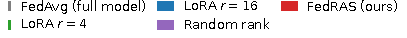
\includegraphics[width=0.45\linewidth]{fig_trainer_legend.pdf}\\[4pt]%
\subfloat[nominal deadline: accuracy]{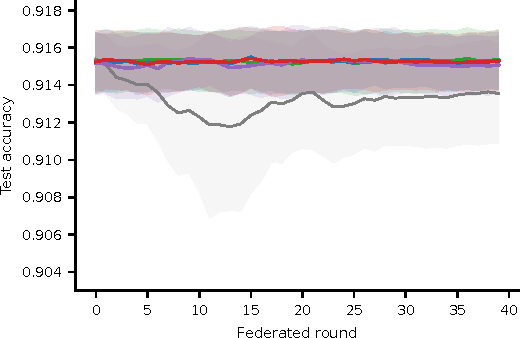
\includegraphics[width=.49\linewidth]{fig_trainer_nominal.pdf}\label{fig:trainermaina}}\hfill%
\subfloat[0.1\,s deadline: accuracy]{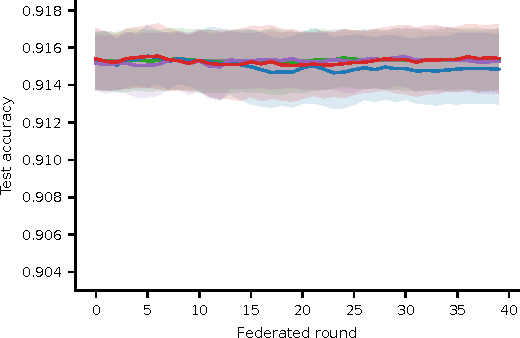
\includegraphics[width=.49\linewidth]{fig_trainer_stress.pdf}\label{fig:trainermainb}}\\[3pt]%
\subfloat[delivered rank per round]{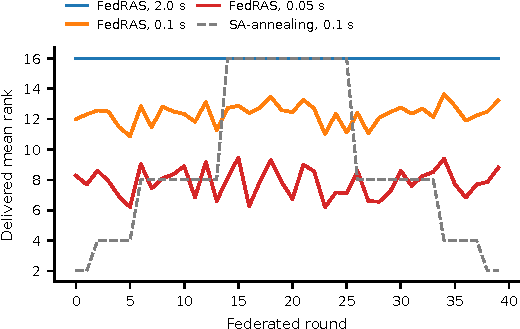
\includegraphics[width=.5035\linewidth]{fig_rank_dynamics.pdf}\label{fig:trainermainc}}\hfill%
\subfloat[accuracy relative to backbone (pp)]{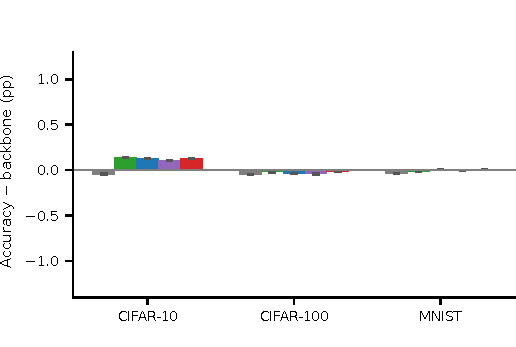
\includegraphics[width=.4743\linewidth]{fig_cross_dataset.pdf}\label{fig:trainermaind}}
\caption{Real-trainer experiments (CIFAR-10, means over seeds). (a)~At the nominal deadline all rank policies hold the pretrained-backbone accuracy. (b)~Under the 0.1\,s deadline all methods remain stable while full-model updates deliver nothing and stay at the backbone. (c)~FedRAS is link-aware: delivered rank holds the provisioned width at the nominal deadline and steps down as the deadline tightens, against the fixed heat--cool path (gray dashed) that the annealing baseline follows regardless of link state. (d)~Final accuracy relative to the per-dataset pretrained backbone; the parity is not CIFAR-10-specific.}
\label{fig:trainermain}
\end{figure*}
\begin{figure*}[pos=!t]
\centering
\subfloat[Timely-delivery ratio]{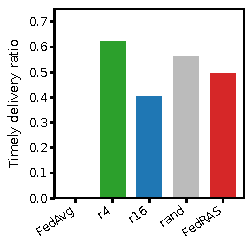
\includegraphics[width=.2465\linewidth]{fig_stresspay_a.pdf}\label{fig:stresspaya}}\hfill%
\subfloat[Attempted MB per round]{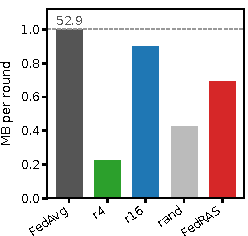
\includegraphics[width=.2465\linewidth]{fig_stresspay_b.pdf}\label{fig:stresspayb}}\hfill%
\subfloat[Timely gain vs.\ rank 16]{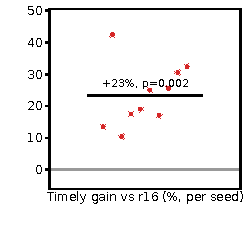
\includegraphics[width=.2465\linewidth]{fig_stresspay_c.pdf}\label{fig:stresspayc}}\hfill%
\subfloat[Byte saving vs.\ rank 16]{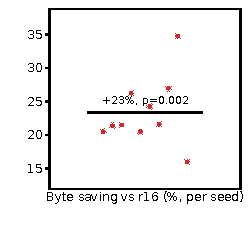
\includegraphics[width=.2465\linewidth]{fig_stresspay_d.pdf}\label{fig:stresspayd}}
\caption{Deadline-stress payoff in the real trainer (CIFAR-10, 0.1\,s deadline, ten seeds). (a)~Timely delivery ratio; full-model updates deliver nothing. (b)~Attempted uplink bytes per round; the FedAvg bar is clipped at 1.0\,MB (true 52.9\,MB, dashed line). (c)~Per-seed relative timely-delivery gain of FedRAS over fixed rank 16: ten of ten pairs positive (per-seed mean $+23\%$; the headline $+22\%$ is the ratio of seed means; Wilcoxon $p=0.002$). (d)~Per-seed byte saving: ten of ten pairs positive ($23\%$, $p=0.002$).}
\label{fig:stresspay}
\end{figure*}

\par
\subsection{Main Experiment: Deadline Ladder and Delivered Capacity}
\label{sec:cmp}
The main experiment answers, in the real trainer, how the scheduler behaves as the deadline tightens: it establishes accuracy parity where the deadline is slack, then tracks every outcome down the deadline ladder and reports the ranking in the single currency of delivered update mass.
\par

\par
\begin{table*}[pos=tbp]
\centering
\rmfamily
\small
\caption{Real-trainer deadline ladder on non-IID CIFAR-10. Nominal and 0.1\,s: ten seeds; 0.05\,s: five seeds. Accuracy is the final-ten-round mean (rounds 30--39, the pre-fixed terminal window); timely-delivery ratio, bytes per round (rounds 30--39, attempted uplink), and mean delivered rank follow the definitions given in the setup. Rounded cells imply $0.49/0.41\approx19.5\%$; the $+22\%$ headline is the ratio of unrounded seed means and the per-seed mean gain is $+23\%$ (\cref{fig:stresspay}c). Per-seed s.d.: timely-delivery ratio $0.03$--$0.06$, MB at most $0.05$ (zero for fixed-rank policies); per-seed tables are in the public repository.}
\label{tab:ladder}
\begin{tblr}
{
columns={co=-1},
cells={valign=m,halign=c},
columns={colsep=2pt},
rows={rowsep=2pt},
rows={ht=0pt},
stretch=0,
hline{1,Z}={wd=.08em},
hline{3}={wd=.05em},
hline{2} = {2-5}{wd=.05em,rightpos=-.6,endpos=true},
hline{2} = {6-9}{wd=.05em,leftpos=-.6,rightpos=-.6,endpos=true},
hline{2} = {10-13}{wd=.05em,leftpos=-.6,endpos=true},
cells={font=\fontsize{9pt}{9pt}},
row{1,2}={font=\bfseries\boldmath\fontsize{9pt}{9pt}},
row{odd[3]}={bg=gray9!35},
cell{1}{2,6,10}={c=4}{},
}
& nominal 2.0\,s & & & & deadline 0.1\,s & & & & deadline 0.05\,s & & & \\
Method & Acc. & Timely & MB & Rank & Acc. & Timely & MB & Rank & Acc. & Timely & MB & Rank \\
FedAvg (full model) & $.9135\pm.0027$ & 0.17 & 52.86 & --- & $.9153\pm.0015$ & 0.00 & 52.86 & --- & $.9147\pm.0016$ & 0.00 & 52.86 & --- \\
FedLoRA $r = 4$ & $.9154\pm.0016$ & 0.75 & 0.23 & 4.0 & $.9154\pm.0016$ & 0.62 & 0.23 & 4 & $.9144\pm.0015$ & 0.57 & 0.23 & 4 \\
FedLoRA $r = 16$ & $.9153\pm.0015$ & 0.73 & 0.90 & 16.0 & $.9149\pm.0019$ & 0.41 & 0.90 & 16 & $.9143\pm.0020$ & 0.27 & 0.90 & 16 \\
Random rank & $.9151\pm.0016$ & 0.76 & 0.42 & 7.3 & $.9153\pm.0017$ & 0.56 & 0.42 & 6.2 & $.9143\pm.0015$ & 0.46 & 0.42 & 5.7 \\
FedRAS (ours) & $.9153\pm.0016$ & 0.73 & 0.90 & 16.0 & $.9154\pm.0018$ & 0.49 & 0.69 & 12.7 & $.9143\pm.0014$ & 0.49 & 0.44 & 8.1 \\
\end{tblr}
\end{table*}
\par
\par
\textbf{Accuracy parity at the nominal deadline.} \cref{tab:ladder} reports ten-seed means and standard deviations after 40 federated rounds on CIFAR-10. All LoRA methods hold the backbone accuracy of 0.914: the primary pair passes the pre-fixed TOST equivalence, and the remaining spreads stay under one standard deviation, whether the rank is fixed at 4, fixed at 16, drawn at random, or selected by the rank rule. Full-parameter updates spend orders of magnitude more bytes per round (\cref{tab:audit}) and lose roughly three quarters of their timely deliveries because their payloads rarely fit the round deadline. The cross-dataset results in \cref{fig:trainermaind} repeat the parity at 0.693 on CIFAR-100 and 0.995 on MNIST at both deadlines, with the stress picture reproduced on both datasets. At the nominal deadline the rank rule selects rank 16 for every client of every round, so FedRAS coincides with fixed rank 16 in bytes and timeliness, and in accuracy up to floating-point nondeterminism; this identity, rather than a tuned advantage, is what the nominal regime is meant to show. \cref{fig:trainermaina} shows the corresponding trajectories, stable over the 40 rounds for every rank policy.
\par
\textbf{Deadline ladder and delivered-rank adaptation.} With parity established at the nominal deadline, we tighten the deadline to $0.1$\,s and $0.05$\,s (\cref{tab:ladder}) and ask where the scheduler moves. Three effects emerge. First, FedRAS downshifts under pressure. Its delivered mean rank falls from 16.0 at the nominal deadline to 12.7 at 0.1\,s and 8.1 at 0.05\,s, where the hazard model \cref{eq:hazard} makes rank-16 payloads marginal. Second, downshifting pays. At 0.1\,s, FedRAS delivers a timely-delivery ratio of 0.49 against 0.41 for fixed rank 16 while transmitting 0.69\,MB against 0.90\,MB, i.e., 23\% fewer bytes (\cref{fig:stresspay}); at 0.05\,s the gap widens to 0.49 against 0.27 timely deliveries at 51\% fewer bytes. In the single currency of delivered update mass the ranking is sharper still: fixed rank 4 leads the timely count (0.62) but its delivered updates carry a quarter of the per-update capacity, so FedRAS delivers 42\% more update mass over the terminal window (mean per-seed gain, $p=0.002$) and 8\% more than fixed rank 16 ($p=0.02$), the most of any evaluated policy. \cref{fig:capview} shows this regime in the single currency itself: every LoRA policy rides the backbone line at parity, FedRAS along the steepest delivered-capacity path, while the full-model curve never leaves it---nothing delivered, no learning. \cref{fig:exchange} assembles the entire exchange behind these numbers: the measured capacity supply, the per-class delivery price, the product peaking at $r^\star$, and the conversion of preserved capacity into accuracy as the backbone weakens. Third, full-model updates collapse completely. Their timely-delivery ratio is 0.00 at both stress deadlines, so not a single full-model update arrives on time in any seed; the stress accuracy of this row is statistically indistinguishable from the per-seed pretrained backbone ($0.915\pm0.002$ across seeds), whose spread explains the nonzero standard deviation. This row is the zero-communication control realized, and read from the availability side it shows what the stress regime is: with nothing delivered, standard federated learning does not degrade---it performs no learning at all, the global model frozen at its broadcast state. The question in this regime is which policies keep a functioning training loop, and rank scheduling is what keeps gradient flow alive at real payload sizes; the LoRA rows meet or exceed the backbone while also moving bytes.
\par
\begin{figure}[pos=tbp]
\centering
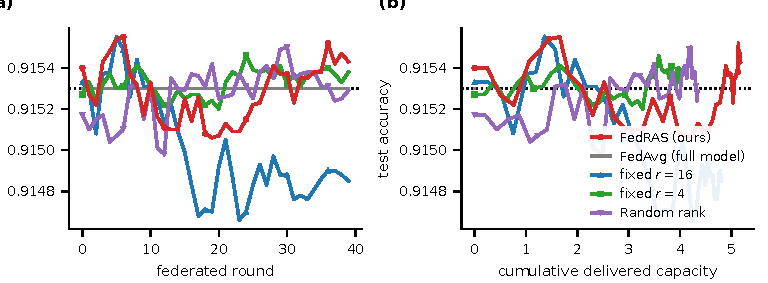
\includegraphics[width=\linewidth]{fig_capview_cifar10_stress.pdf}
\caption{The strong-backbone stress regime in the single currency. (a)~Accuracy trajectories and (b)~accuracy against cumulative delivered update mass (terminal window, rounds 30--39, as everywhere): every LoRA policy sits at backbone parity, FedRAS reaches it along the steepest capacity path, and the flat full-model curve is the zero-communication control realized---nothing delivered, no learning.}
\label{fig:capview}
\end{figure}
\begin{figure*}[pos=tbp]
\centering
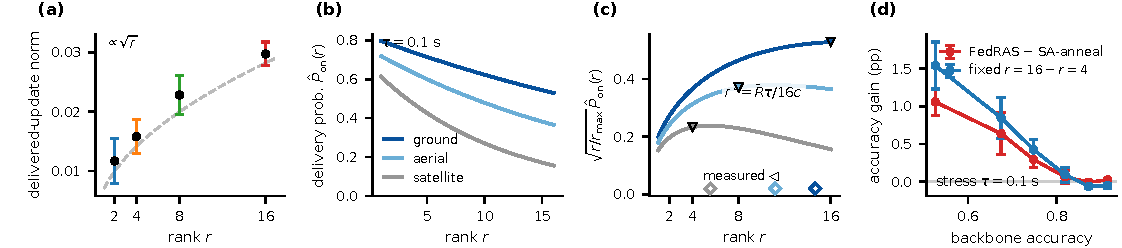
\includegraphics[width=\linewidth]{fig_exchange.pdf}
\caption{The capacity--delivery exchange in one picture. (a)~Supply: the measured delivered-update norm grows with the square root of the rank (the anchor of \cref{eq:cap}). (b)~Price: the payload-conditioned delivery probability of \cref{eq:hazard} per SAGIN link class at the 0.1\,s deadline, at each class's median rate and mean mobility. (c)~Law: the product $\sqrt{r/r_{\max}}\,\hat P_{\rm on}(r)$ peaks at the closed form $r^\star$ of \cref{eq:rstar} (triangles; ground peaks at the provisioned width), and the diamonds are the trainer's measured per-class delivered ranks in the grouped-profile stress runs, tracking the peaks. (d)~Conversion: the accuracy value of preserved capacity as the backbone weakens (\cref{sec:weakbb}); the gain vanishes on the strong backbone and grows as adaptation becomes scarce.}
\label{fig:exchange}
\end{figure*}
\cref{fig:rstar} validates the closed form $r_i^\star$ of \cref{eq:rstar} against the trainer's actual assignments in the grouped-profile stress runs; the nearest-candidate reading of $r_i^\star$ reproduces the assigned rank on about three quarters of two thousand client--round points, and the remainder sits one step below at candidate boundaries, where the discrete argmax is slightly conservative.
\par
\begin{figure}[pos=tbp]
\centering
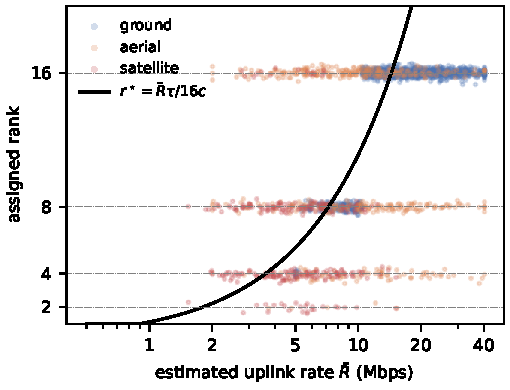
\includegraphics[width=\linewidth]{fig_rstar_validation.pdf}
\caption{The closed form \cref{eq:rstar} against the trainer's actual assignments in the grouped-profile stress runs (0.1\,s, five seeds, 2000 client--round points, one dot per assignment with vertical jitter). Assignments track $r_i^\star$ across all three link classes; the nearest-candidate reading of the closed form reproduces the assigned rank on about three quarters of the points, and the remainder sits one step below at candidate boundaries, where the discrete argmax is slightly conservative.}
\label{fig:rstar}
\end{figure}

\textbf{Delivered-update norms.} The capacity law is anchored in measurement: the trainer logs the mean Frobenius norm of each round's delivered updates, and across the full candidate set the measured growth tracks the $\sqrt{r}$ law of \cref{eq:cap} ($2.5\times$ from rank 2 to 16 against $2.8\times$ predicted, and $1.9\times$ from rank 4 to 16 against $2.0\times$, with the stress series coinciding with the nominal one; \cref{fig:normlaw}). The measured norm curve anchors the shape of \cref{eq:cap}; the exponent choice is bounded by the capacity-exponent sweep of the sensitivity study.
\par
\begin{figure}[pos=tbp]
\centering
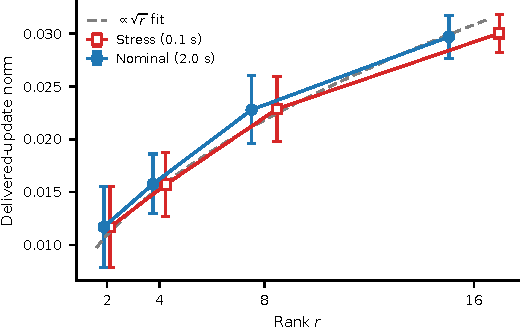
\includegraphics[width=\linewidth]{fig_normlaw.pdf}
\caption{Delivered-update norm vs.\ rank on CIFAR-10 (mean over delivered rounds; five seeds per point, error bars are one standard deviation). The measured growth ($2.5\times$ from rank 2 to 16, $1.9\times$ from rank 4 to 16) tracks the square-root capacity law of \cref{eq:cap} ($2.8\times$ and $2.0\times$) rather than linear payload growth ($8\times$ and $4\times$); the nominal and stress series coincide.}
\label{fig:normlaw}
\end{figure}


\textbf{Why downshifting dominates.} Payload grows linearly in the rank while delivery probability falls convexly once transmission time approaches the deadline, so the scheduler buys delivery probability where it is cheap and holds high rank where it is free. In this regime the binding constraint on learning is delivery, not adaptation capacity, which is why the delivered rank moves while accuracy stays at parity.
\par
\textbf{Mechanism and replication.} Accuracy spreads remain small and inside the pre-fixed equivalence margin, with the primary pair passing the TOST test and further pairs read as descriptive parity; the scheduling metrics are where the methods separate (\cref{fig:trainermainb,fig:trainermainc}). All headline differences replicate across the ten paired seeds at conventional significance levels, with the statistics fixed in advance.
\par
\subsection{Adaptive Tasks and the Capacity-Conversion Law}
\label{sec:weakbb}
The main experiment separated the methods in delivered adaptation capacity while leaving accuracy at parity on the strong backbone. This section locates where that capacity turns into accuracy: first on tasks whose backbone genuinely needs adaptation, then across a backbone-quality sweep that measures the conversion boundary itself.
\par
\textbf{Does communication buy learning?} Two adaptive tiers answer this, each with the zero-communication control of the metrics made explicit. On the disjoint-pretraining weak backbone (backbone accuracy 0.365 on the deployment test), forty federated rounds buy roughly three points of accuracy: 0.400 for fixed rank 16 and joint A/B, 0.396 for FedRAS, 0.378 for the annealed schedule, against 0.376 for the fixed low rank (\cref{fig:adaptweakdisj}a); under the stress deadline FedRAS retains almost all of this gain while beating fixed rank 16 on timely delivery (0.49 vs 0.41) at fewer bytes. On the tiny-ViT tier with covariate-shifted clients (backbone 0.727 on the shifted test), every LoRA policy recovers about one point (FedRAS 0.735, fixed rank 16 0.737), full-model updates deliver nothing at the 0.5\,s deadline and stay at the backbone, and FedRAS holds the recovered accuracy with 48\% more timely updates than fixed rank 16 at 39\% fewer bytes (ten of ten paired seeds, $p=0.002$; \cref{fig:adaptvit}); the right-hand panels of both figures re-plot the same trajectories against cumulative uplink bytes, the cost view the adaptive question asks for. The CNN covariate-shift tier marks the boundary of adapter recovery: all rank policies sit within half a point of the shifted backbone (0.824), so under this shift the adapters preserve rather than recover accuracy while the scheduler still wins the delivery side (0.49 vs 0.41 timely, 0.69 vs 0.90\,MB). Communication pays exactly where the backbone needs adaptation, and scheduling preserves the payment under stress.
\par
\begin{figure*}[pos=tbp]
\centering
\subfloat[weak backbone, disjoint pretraining, 0.1\,s deadline]{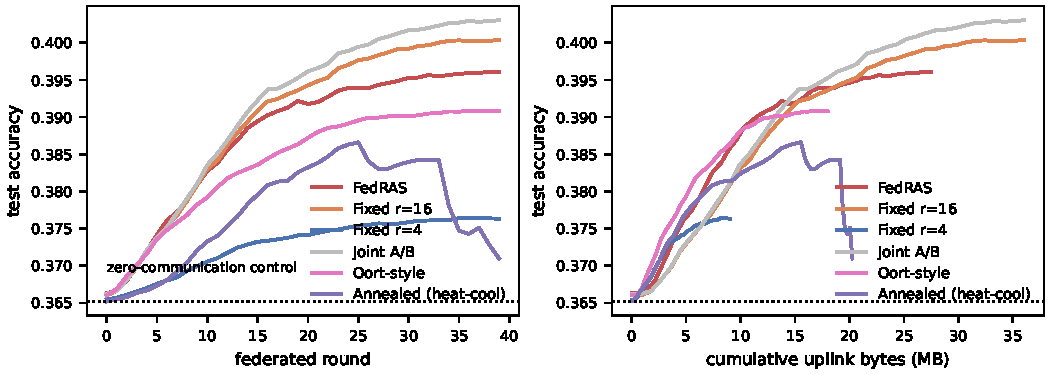
\includegraphics[width=.49\linewidth]{fig_adapt_weakdisj.pdf}\label{fig:adaptweakdisj}}\hfill%
\subfloat[tiny ViT, covariate shift, 0.5\,s deadline]{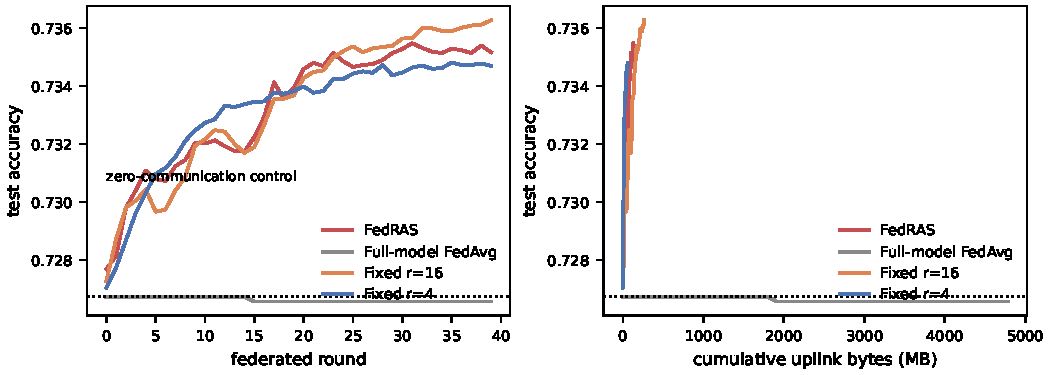
\includegraphics[width=.49\linewidth]{fig_adapt_vitshift.pdf}\label{fig:adaptvit}}
\caption{Adaptive-task evidence, accuracy vs round (left of each panel) and vs cumulative uplink bytes (right); the dotted line is the zero-communication control (frozen backbone on the deployment distribution), and the flat full-model curve in (b) is that control realized: nothing delivered at the stress deadline. (a)~Disjoint-pretraining weak backbone: communication buys about three points, FedRAS keeps nearly all of it at stress. (b)~Shifted tiny ViT: LoRA recovers about one point, and FedRAS preserves it with $+48\%$ timely and $-39\%$ bytes against fixed rank 16 ($p=0.002$).}
\label{fig:adapt}
\end{figure*}
\begin{figure*}[pos=!b]
\centering
\subfloat[Nominal deadline]{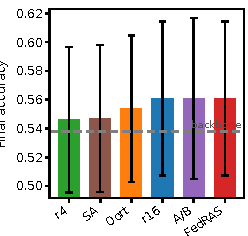
\includegraphics[width=.2465\linewidth]{fig_weakbb6_a.pdf}\label{fig:weakbba}}\hfill%
\subfloat[Stress deadline (0.1\,s)]{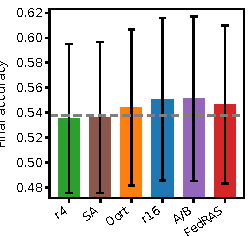
\includegraphics[width=.2465\linewidth]{fig_weakbb6_b.pdf}\label{fig:weakbbb}}\hfill%
\subfloat[FedRAS vs.\ SA-anneal, per seed]{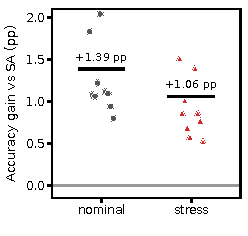
\includegraphics[width=.2465\linewidth]{fig_weakbb6_c.pdf}\label{fig:weakbbc}}\hfill%
\subfloat[Attempted MB per round]{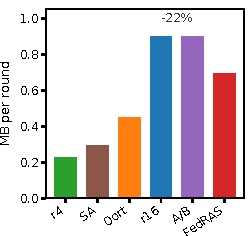
\includegraphics[width=.2465\linewidth]{fig_weakbb6_d.pdf}\label{fig:weakbbd}}
\caption{Weak-backbone capacity payoff with the literature schedules (one-epoch pretrain, ten seeds). (a)~At the nominal deadline the high-rank policies lead low-rank operation by about 1.5 points and FedRAS coincides with rank 16; the dashed line marks the pretrained backbone. (b)~Under the 0.1\,s deadline the link-oblivious SA schedule drops onto the low-rank trajectory. (c)~Paired per-seed accuracy differences against the SA schedule: every seed is positive at both deadlines (ten of ten, $p = 0.002$). (d)~FedRAS transmits $23\%$ fewer bytes than the accuracy-matching rank-16 and joint A/B policies.}
\label{fig:weakbb}
\end{figure*}
\textbf{The capacity-conversion law.} The strong-backbone regime makes adaptation capacity free, so preserving rank carries no measurable benefit there. To measure exactly where that stops being true, we sweep the backbone itself: one, two, three, five, ten, and thirty pretraining epochs yield measured backbone accuracies of 0.53, 0.68, 0.75, 0.82, 0.87, and 0.91 on the deployment test, and every tier runs the full six-method family with ten paired seeds at both deadlines. Two curves result (\cref{fig:exchange}d). The nominal coupling, fixed rank 16 over fixed rank 4, decays monotonically from $+1.5$ points at backbone accuracy 0.53 to zero at 0.87, and the scheduler's realized gain over the link-oblivious annealed schedule tracks it: $+1.1$ points at 0.53 ($p=0.002$), $+0.6$ at 0.68, $+0.3$ at 0.75 (both $p\le0.05$), statistical zero from 0.82 upward---capturing about two-thirds to three-quarters of the available coupling at every tier where coupling exists. The conversion boundary is sharp and operational: \emph{delivered capacity converts into accuracy once the backbone falls below roughly 0.8, and the conversion grows as adaptation becomes scarce.}
\par
\textbf{The weakest tier in detail.} At the one-epoch tier (backbone accuracy $0.534$, mean over ten seeds), federated adaptation improves on the pretrained weights by roughly two points, and the rank--accuracy coupling appears at the nominal deadline (\cref{fig:weakbba}), where rank 16 reaches $0.561$ against rank 4's $0.546$ over ten paired seeds ($+1.5$ points, Wilcoxon $p = 0.002$), with FedRAS coinciding with rank 16. Under the 0.1\,s deadline the coupling persists and the scheduler prices it without any retuning (\cref{fig:weakbbb}): FedRAS holds a delivered rank of 12.8, finishes $1.1$ points above rank 4 (ten of ten pairs), while trading $0.4$ points to fixed rank 16 for a $22\%$ higher timely-delivery ratio and $23\%$ fewer bytes (\cref{fig:weakbbd}).
\par
\begin{table*}[pos=tbp]
\centering
\rmfamily
\small
\caption{No static policy is right everywhere. Four regimes (deadline $\times$ backbone quality), four policies, ten paired seeds each; every cell reports the accuracy gap to the best policy in that regime (percentage points), the delivered update mass (terminal-window delivered capacity, \% of the regime best), and the timely-delivery ratio (\% of best). Fixed $r{=}4$ holds the timely lead everywhere yet pays about 1.5 points in the weak regimes and never delivers more than three quarters of the best capacity; fixed $r{=}16$ owns the nominal regimes but loses 35\% of its deliveries at stress; the annealed schedule matches FedRAS on the strong backbone---low rank is adequate exactly when capacity is free---and drops 1.4--1.5 points precisely where capacity matters. FedRAS is the only policy whose worst cell is bounded at 0.41 points while holding the full delivered capacity of its regime throughout, because it reads which regime it is in from the link instead of fixing the answer offline.}
\label{tab:failures}
\begin{tblr}
{
columns={co=-1},
cells={valign=m,halign=c},
columns={colsep=3pt},
rows={rowsep=2pt},
rows={ht=0pt},
stretch=0,
hline{1,Z}={wd=.08em},
hline{2}={wd=.05em},
cells={font=\fontsize{9pt}{9pt}},
row{1}={font=\bfseries\boldmath\fontsize{9pt}{9pt}},
row{even[2]}={bg=gray9!35},
cell{1}{1}={halign=l},
cell{2}{1}={halign=l},
cell{3}{1}={halign=l},
cell{4}{1}={halign=l},
cell{5}{1}={halign=l},
}
Policy & nominal / strong & stress / strong & nominal / weak & stress / weak \\
Fixed $r{=}4$ & $-0.0$ / 54\% / 100\% & $-0.0$ / 72\% / 100\% & $-1.5$ / 55\% / 100\% & $-1.5$ / 73\% / 100\% \\
Fixed $r{=}16$ & $-0.0$ / 100\% / 97\% & $-0.1$ / 93\% / 65\% & $-0.0$ / 100\% / 97\% & $-0.0$ / 92\% / 65\% \\
SA anneal & $-0.0$ / 65\% / 100\% & $-0.0$ / 83\% / 99\% & $-1.4$ / 66\% / 100\% & $-1.5$ / 84\% / 99\% \\
FedRAS & $-0.0$ / 100\% / 97\% & $-0.0$ / 100\% / 80\% & $-0.0$ / 100\% / 97\% & $-0.4$ / 100\% / 80\% \\
\end{tblr}
\end{table*}
\par
\textbf{No static policy is right everywhere.} \cref{tab:failures} assembles the four regimes the paper has measured. Each static policy is optimal in one of them---by construction or by luck of the backbone---and pays elsewhere: the low rank pays accuracy where capacity matters, the high rank pays delivery once deadlines bind, and the training-signal schedule cannot see the difference. The link-conditioned rule is the only one that is near-optimal in every regime without being told which regime it is in.
\par
\subsection{Comparison With Baselines}
\label{sec:cmp2}
The comparison places FedRAS against fixed-rank and full-model policies, external schedules in both stylized and faithful variants, simple network-aware rules, and the heuristics at 500-client scale, under identical partitions, link traces, and seed protocol.
\par

\par
\textbf{Against low-rank baselines.} Across \cref{tab:ladder,tab:extbaselines}, the remaining policies sit on one delivery--capacity trade-off: random-rank, Oort-style, and annealed schedules deliver \emph{more} timely updates at \emph{fewer} bytes than FedRAS (\cref{fig:trainermainc}), but at delivered ranks of 5.0--8.0 against FedRAS's 12.7. What FedRAS keeps on this trade-off is adaptation capacity. Whether preserved capacity converts into accuracy in regimes where capacity matters is tested with the weak-backbone study.

\label{sec:extbase}
\textbf{Literature-mechanism baselines.} \cref{tab:extbaselines} reports the three external baselines of the setup in the real trainer. The link-oblivious annealing schedule settles at low rank and therefore buys timely delivery at the lowest byte cost among the baselines, but it cannot increase rank when links improve. The Oort-style selector acts on selection only and leaves the rank fixed. Joint A/B training matches frozen-factor training at the adopted learning rate, and the ablations find no stability separation at an elevated learning rate either, so the case for the frozen factor rests on exactness and upload reduction rather than on an observed stability gap.
\par
\textbf{Compression baseline.} A fixed rank-16 policy with an FP16 upload (two bytes per parameter, real round-trip quantization on delivery) halves the payload and, at the 0.1\,s deadline, delivers 0.55 timely updates at 0.45\,MB, more timely updates than any FP32 schedule at the same rank (\cref{tab:extbaselines}). Stacking FedRAS on the same format extends the gain: FedRAS-FP16 beats FP16 rank 16 in ten of ten seed pairs ($+12\%$ timely, $23\%$ fewer bytes, $p = 0.002$ each) at equal accuracy. Compression re-prices every rank; the scheduler re-optimizes the assignment under the prices that hold.
\par
\par
\begin{table*}[pos=tbp]
\centering
\rmfamily
\small
\caption{External baselines in the real trainer, ten seeds. The FP16 rows use the FP16 serialized sizes of \cref{tab:audit}. The joint A/B plain row is computed at the $B$-only payload for comparability; the true-payload row bills it end-to-end at the audited $A{+}B$ size (1.64\,MB per ten-client round at rank 16). The near-neighbor rows (expected latency, SVD allocation, monotone annealing) are faithful-style re-implementations of the cited mechanisms under the shared protocol.}
\label{tab:extbaselines}
\begin{tblr}
{
columns={co=-1},
cells={valign=m,halign=c},
columns={colsep=6pt},
rows={rowsep=2pt},
rows={ht=0pt},
stretch=0,
hline{1,Z}={wd=.08em},
hline{3}={wd=.05em},
hline{2} = {2-5}{wd=.05em,rightpos=-.4,endpos=true},
hline{2} = {6-9}{wd=.05em,leftpos=-.4,endpos=true},
cells={font=\fontsize{9pt}{9pt}},
row{1,2}={font=\bfseries\boldmath\fontsize{9pt}{9pt}},
row{odd[3]}={bg=gray9!35},
cell{1}{2,6}={c=4}{},
}
& nominal 2.0\,s & & & & deadline 0.1\,s & & & \\
Method & Acc. & Timely & MB & Rank & Acc. & Timely & MB & Rank \\
SA-FedLoRA-style annealing & $.9152\pm.0017$ & 0.75 & 0.29 & 5.2 & $.9152\pm.0016$ & 0.62 & 0.29 & 5.2 \\
Annealing, monotone shrink & $.916\pm.001$ & 0.75 & 0.21 & 3.8 & $.916\pm.002$ & 0.63 & 0.21 & 3.8 \\
Rate threshold & $.916\pm.001$ & 0.74 & 0.67 & 11.8 & $.916\pm.002$ & 0.54 & 0.67 & 11.2 \\
Oort-style utility, fixed rank & $.9150\pm.0020$ & 0.76 & 0.45 & 8.0 & $.9150\pm.0019$ & 0.54 & 0.45 & 8.0 \\
Expected-latency rule (after ROBA/TSFA) & $.915\pm.001$ & 0.73 & 0.90 & 16.0 & $.915\pm.001$ & 0.45 & 0.79 & 14.4 \\
SVD rank allocation (after FedARA) & $.915\pm.001$ & 0.75 & 0.11 & 2.0 & $.915\pm.001$ & 0.68 & 0.11 & 2.0 \\
Joint A/B, plain averaging & $.9152\pm.0016$ & 0.73 & 0.90 & 16 & $.9149\pm.0019$ & 0.40 & 0.90 & 16 \\
Joint A/B, true $A{+}B$ payload & $.915\pm.002$ & 0.70 & 1.64 & 16 & $.915\pm.001$ & 0.28 & 1.64 & 16 \\
FedLoRA $r = 16$, FP16 upload & $.9146\pm.0013$ & 0.74 & 0.45 & 16 & $.9149\pm.0015$ & 0.55 & 0.45 & 16 \\
FedRAS, FP16 upload & $.9146\pm.0011$ & 0.74 & 0.45 & 16 & $.9143\pm.0017$ & 0.62 & 0.35 & 12.5 \\
\end{tblr}
\end{table*}
\par
\par

\textbf{Near-neighbor mechanisms.} Two literature-mechanism re-implementations complete the comparison (\cref{tab:extbaselines}). The expected-latency rule (after ROBA/TSFA) reads the same estimated rates as FedRAS but admits the largest rank whose \emph{expected} transmission time meets the deadline; at 0.1\,s it holds rank 14.4 on average and delivers 0.45 at 0.79\,MB, link-aware, but it prices neither loss nor admission, so it pays near-full-rank bytes for mid-rank delivery. The SVD rank allocation (after FedARA) follows the aggregated update's energy and settles at rank 2.0 with 0.68 timely at 0.11\,MB, the training-side counterpart of the delivery-only policy: timely and capacity-poor. The faithful monotone annealing lands with its stylized twin (0.63 vs 0.62 timely at 0.21\,MB), and the rate threshold tracks FedRAS's network columns through a fixed two-rank split. On the weak backbone every link-aware rule beats the link-oblivious schedules, expected-latency 0.565, fixed rank 16 0.551, FedRAS 0.547, against 0.536--0.544 for annealing and Oort-style, and the family result matches the positioning of \cref{tab:rwcompare}: pricing the link at all is what matters, and within the link-aware family the delivery-probability pricing buys the most timely updates at the fewest bytes (FedRAS: 0.49 timely, 0.69\,MB) while the expected-latency pricing retains about two points more accuracy by holding wider ranks at more bytes, the capacity--delivery trade again, now between pricing philosophies.
\textbf{Against the literature schedules.} The same paired runs place the external baselines in this regime. The SA-FedLoRA-style annealing schedule sits on the low-rank trajectory and finishes $1.3$ points below FedRAS at the nominal deadline and $1.1$ points below under stress (ten of ten seeds each, $p = 0.002$; \cref{fig:weakbbc}): its link-oblivious heat--cool path spends rounds at low rank exactly when the backbone needs capacity. The scheduler holds the rank level that delivers the accuracy; an annealing path that ended hot would recover capacity but lose the timely delivery that motivates annealing, which is the trade-off the architecture resolves. The Oort-style selector, fixed at the mid rank, lands in between, $0.7$ points below FedRAS at the nominal deadline (eight of ten pairs, $p = 0.037$) and indistinguishable under stress. Joint A/B training at the full width matches the rank-16 accuracy at both deadlines; billed end-to-end at its true $A{+}B$ payload its timely-delivery ratio at 0.1\,s falls to 0.28 at 1.64\,MB per round (\cref{tab:extbaselines}). Preserved capacity therefore converts into accuracy when the backbone is weak enough to need adaptation, and against link-oblivious rank schedules the conversion is a direct accuracy win, which is the regime in which a rank scheduler has a reason to exist.
\par
\textbf{Cross-tier summary.} Taken together, the two evaluation tiers give a consistent picture. Rank choice does not measurably change accuracy for the frozen backbone at the 40-round horizon, and the headline comparisons against fixed rank 16 pass the TOST equivalence test fixed in advance at the $\pm0.5$ percentage-point margin; an offline control that ignores delivery modeling entirely and trains on every scheduled update reaches $0.913\pm0.002$ at the nominal deadline, close to the backbone's $0.914$, separating learning capacity from delivery feasibility. The methods instead separate in delivered adaptation capacity: FedRAS holds high ranks on healthy links and downshifts under pressure, full-model updates collapse once deadlines bind at real payload sizes, and the exact scheduler pays through admission over the candidate pool rather than in-cohort rank allocation (\cref{prop:cohort}). Two stress tests bound these claims from both sides: the delivered-capacity gains survive stacking on an FP16 codec, and a weaker backbone reveals accuracy value in the preserved capacity exactly where the strong-backbone regime shows none. These tests rest on ten-seed replications of the headline trainer regimes; they support the stated delivered-capacity comparisons and the accuracy equivalence. The discussion that follows interprets these findings, states their scope conditions, and translates them into deployment guidance.
\subsection{Ablation and Sensitivity}
\label{sec:abl}
The ablation first removes each mechanism of the architecture and then varies the solver regime, separating the value of candidate-pool widening from the value of exact solving under a binding byte budget.
\par
\begin{table}[pos=tbp]
\centering
\rmfamily
\small
\caption{Ablation study of the real trainer (nominal deadline; the rank-mask row is at 0.1\,s). Seeds as in the protocol; Timely and MB follow the setup definitions and expose the behavioral effect each mechanism produces (removing the capacity term collapses the schedule to minimum rank, i.e., 0.11\,MB). Min.\ is the minimum over rounds of the per-round seed-mean accuracy in the elevated-learning-rate check (lr 0.02).}
\label{tab:ablation}
\begin{tblr}
{
columns={co=-1},
cells={valign=m,halign=c},
columns={colsep=5pt},
rows={rowsep=2pt},
rows={ht=0pt},
stretch=0,
hline{1,Z}={wd=.08em},
hline{2,6}={wd=.05em},
cells={font=\fontsize{9pt}{9pt}},
row{1}={font=\bfseries\boldmath\fontsize{9pt}{9pt}},
row{even[2]}={bg=gray9!35},
}
Configuration & Accuracy & Timely & MB & Min. \\
Full system (ours) & $.9153\pm.0015$ & 0.73 & 0.90 & --- \\
w/o capacity term & $.9145\pm.0015$ & 0.75 & 0.11 & --- \\
w/o frozen $A$ (joint A/B) & $.9152\pm.0016$ & 0.73 & 0.90 & --- \\
w/o rank mask (random ranks, 0.1\,s) & $.9145\pm.0016$ & 0.58 & 0.42 & --- \\
w/o server momentum & $.9143\pm.0012$ & 0.74 & 0.90 & --- \\
frozen $A$, lr 0.02 & $.9130\pm.0012$ & 0.74 & 0.90 & 0.913 \\
joint A/B, lr 0.02 & $.9130\pm.0011$ & 0.74 & 0.90 & 0.912 \\
\end{tblr}
\end{table}
\par
\textbf{Ablation analysis.} \cref{tab:ablation} reports mechanism ablations at the nominal deadline. In the parity regime all accuracy differences sit inside the equivalence margin (descriptive for ablation pairs); the mechanisms act on scheduling behavior and aggregation correctness. Removing the capacity term collapses FedRAS to the minimum rank, the degenerate delivery-only policy that the capacity term exists to prevent; its capacity cost is invisible at nominal deadlines but material in the simulator, where reliability-only optimization loses 28 points of utility against rank 16 (\cref{tab:scalemain}(a)). Removing server momentum is accuracy-neutral here. The rank mask itself is network-metric-neutral at fixed rank policy: with the random-rank rule at the 0.1\,s deadline, masked and unmasked aggregation give 0.9145 and 0.9145 final accuracy with identical byte and timeliness profiles. The mask is nonetheless what keeps heterogeneous-rank aggregation per-slice exact whenever ranks mix, as \cref{prop:agg} states. Under the weak backbone at the 0.1\,s deadline, where delivered ranks mix around 12.7 and capacity affects accuracy, masked averaging finishes $1.4$ points above the unified-denominator (unmasked) rule on identical seeds (0.547 vs 0.533), and the $W_j=0$ fallback is itself load-bearing: holding the previous server state at uncovered columns finishes another $1.7$ points above the pull-to-zero default (0.564, five seeds, with half the seed variance). The aggregation choices are empirically decisive in exactly the regime the architecture targets.
\par
\textbf{Stability at elevated learning rate.} Under the elevated learning rate of 0.02, the frozen-factor rule and joint A/B training are statistically indistinguishable, with final accuracies of 0.9130 and 0.9132 and transient minima of 0.913 and 0.912 across rounds and seeds. The frozen-factor rule is therefore justified by the exactness of \cref{prop:agg} and by its single-factor uploads, not by an empirical stability margin at this scale.
\par
\textbf{Binding budget.} With the trainer budget tightened to 0.4\,MB, four rank-16 grid costs, so the cap and the budget interact, exact solving pays in real training: the full dynamic program delivers a timely-delivery ratio of 0.69 at 0.34\,MB with delivered rank 6.0, the value greedy 0.57 at 0.36\,MB (the DP wins ten of ten paired seeds, $p=0.002$), and the value-per-byte greedy 0.78 at 0.11\,MB by collapsing to rank 2.0, buying timeliness with a third of the DP's delivered capacity. The unchecked per-client rule transmits 0.69\,MB, violating the budget it does not model, and fixed rank 16 delivers 0.41. Exactness therefore earns its cost precisely where the solver study predicted: under a binding budget, the admission-coupled value that per-client orderings leave behind is real, measurable, and collected by the DP.

\label{sec:dpvfair}
\textbf{Arms under evaluation.} To attribute the value of exact scheduling, the three arms defined in the setup are compared in the real trainer, over ten seeds at the nominal deadline and five seeds under stress. The full grid arm solves the GridDP assignment over the entire 20-client population under the participation cap and a 1.0\,MB budget, which equals ten rank-16 grid costs, so the budget binds only through downshifting or skipping. The same-cohort arm draws the identical cohort as the fair-cohort arm and restricts the same dynamic program to those candidates.
\par
\textbf{Where exactness pays.} \cref{tab:arms} yields a clean decomposition. At the nominal deadline, the same-cohort DP coincides exactly with the per-client rule, as \cref{prop:cohort} predicts; the full DP's timely-delivery gain ($+9$ percentage points) comes entirely from admission over the wider candidate pool. Under the 0.1\,s deadline the pattern persists: the in-cohort DP matches the per-client rule, while the full DP delivers more timely updates at proportionally more bytes. The two in-cohort arms share the cohort draw and the link traces by construction, so their assignments coincide; their delivered-rank cells (12.8 vs 12.7) differ only through the independent delivery coin flips of separate runs, sampling noise on identical schedules, not a scheduling difference. Exactness therefore pays through admission control over a heterogeneous pool, not through rank allocation inside a cohort (\cref{prop:cohort}). This delimits when full grid scheduling is worth its coordination cost.
\par
\par
\begin{table*}[pos=tbp]
\centering
\rmfamily
\small
\caption{Scheduling arms in the real trainer (1.0\,MB budget; the FedLoRA $r = 16$ reference is in \cref{tab:ladder}). Nominal: ten seeds; stress 0.1\,s: five seeds.}
\label{tab:arms}
\begin{tblr}
{
columns={co=-1},
cells={valign=m,halign=c},
columns={colsep=6pt},
rows={rowsep=2pt},
rows={ht=0pt},
stretch=0,
hline{1,Z}={wd=.08em},
hline{3}={wd=.05em},
hline{2} = {2-5}{wd=.05em,rightpos=-.4,endpos=true},
hline{2} = {6-9}{wd=.05em,leftpos=-.4,endpos=true},
cells={font=\fontsize{9pt}{9pt}},
row{1,2}={font=\bfseries\boldmath\fontsize{9pt}{9pt}},
row{odd[3]}={bg=gray9!35},
cell{1}{2,6}={c=4}{},
}
& nominal 2.0\,s, ten seeds & & & & stress 0.1\,s, five seeds & & & \\
Arm & Acc. & Timely & MB & Rank & Acc. & Timely & MB & Rank \\
Full DP (grid assignment) & $.9151\pm.0017$ & 0.82 & 0.90 & 16.0 & $.9139\pm.0009$ & 0.55 & 0.87 & 15.3 \\
Same-cohort DP & $.9152\pm.0018$ & 0.73 & 0.90 & 16.0 & $.9139\pm.0014$ & 0.51 & 0.70 & 12.8 \\
Fair cohort (FedRAS rule) & $.9153\pm.0015$ & 0.73 & 0.90 & 16.0 & $.9154\pm.0018$ & 0.51 & 0.70 & 12.7 \\
\end{tblr}
\end{table*}
\par
\par
\begin{table*}[pos=tbp]
\centering
\rmfamily
\small
\caption{Experiments at 500-client scale (five seeds unless noted). (a) Scheduler simulation across regimes; the utility column is the bounded scheduling utility defined in the setup and must not be read as dataset accuracy, MB is the attempted uplink payload of admitted clients in the final round billed on the same 0.01\,MB ceiling grid as budget admission, and FedAvg refers to full-model updates at their real serialized size. (b) Solver study with $K = 25$ and 30 instances per cell on the identical ceiling grid; the table reports heuristic objective loss relative to the grid-based DP and DP runtime.}
\label{tab:scalemain}
\textsf{(a) Scheduler simulation across regimes}
\par\vspace{2pt}
\begin{tblr}
{
columns={co=-1},
cells={valign=m,halign=c},
columns={colsep=6pt},
rows={rowsep=2pt},
rows={ht=0pt},
stretch=0,
hline{1,Z}={wd=.08em},
hline{3}={wd=.05em},
hline{2} = {2-4}{wd=.05em,rightpos=-.2,endpos=true},
hline{2} = {5-7}{wd=.05em,leftpos=-.2,rightpos=-.2,endpos=true},
hline{2} = {8-10}{wd=.05em,leftpos=-.2,endpos=true},
cells={font=\fontsize{9pt}{9pt}},
row{1,2}={font=\bfseries\boldmath\fontsize{9pt}{9pt}},
cell{Z}{5,8}={font=\bfseries\boldmath\fontsize{9pt}{9pt}},
row{odd[3]}={bg=gray9!35},
cell{1}{2,5,8}={c=3}{},
}
& Nominal 2.0\,s & & & Deadline 0.1\,s & & & Budget 1.2\,MB & & \\
Method & Utility & Timely & MB & Utility & Timely & MB & Utility & Timely & MB \\
FedAvg (full) & .310 & .34 & 26.5 & .093 & .00 & 26.5 & .093 & .00 & 0.0 \\
$r = 4$ & .744 & .75 & 0.8 & .689 & .64 & 0.8 & .744 & .75 & 0.8 \\
$r = 16$ & .914 & .73 & 2.5 & .763 & .42 & 2.5 & .797 & .76 & 1.2 \\
Random & .816 & .75 & 1.3 & .709 & .57 & 1.3 & .803 & .75 & 1.2 \\
Reliability-only & .635 & .76 & 0.5 & .606 & .70 & 0.5 & .635 & .76 & 0.5 \\
SA-annealing & .842 & .76 & 0.5 & .730 & .70 & 0.5 & .796 & .76 & 0.5 \\
FedRAS (ours) & .914 & .73 & 2.5 & .781 & .50 & 2.0 & .797 & .76 & 1.2 \\
\end{tblr}
\par\vspace{3pt}
\textsf{(b) Solver study}
\par\vspace{2pt}
\begin{tblr}
{
columns={co=-1},
cells={valign=m,halign=c},
columns={colsep=6pt},
rows={rowsep=2pt},
rows={ht=0pt},
stretch=0,
hline{1,Z}={wd=.08em},
hline{2}={wd=.05em},
cells={font=\fontsize{9pt}{9pt}},
row{1}={font=\bfseries\boldmath\fontsize{9pt}{9pt}},
row{even[2]}={bg=gray9!35},
}
Deadline (s) & Budget (MB) & Greedy val/byte & Greedy value & Cohort myopic & Fixed $r = 16$ & DP time (ms) \\
2.0 & 30 & 63.6\% & 0.0\% & 40.9\% & 0.0\% & 421 \\
2.0 & 4 & 63.6\% & 0.0\% & 40.9\% & 0.0\% & 51 \\
2.0 & 1.2 & 47.8\% & 28.4\% & 48.9\% & 28.4\% & 23 \\
1.0 & 30 & 62.7\% & 0.0\% & 40.0\% & 0.0\% & 415 \\
1.0 & 4 & 62.7\% & 0.0\% & 43.0\% & 0.0\% & 51 \\
1.0 & 1.2 & 47.3\% & 29.3\% & 48.3\% & 29.3\% & 23 \\
0.1 & 30 & 52.8\% & 0.0\% & 51.9\% & 0.0\% & 415 \\
0.1 & 4 & 52.6\% & 0.0\% & 52.0\% & 0.0\% & 51 \\
0.1 & 1.2 & 41.0\% & 36.0\% & 54.8\% & 36.0\% & 23 \\
\end{tblr}
\end{table*}
\begin{figure}[pos=!ht]
\centering
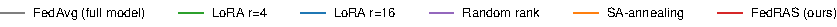
\includegraphics[width=\columnwidth]{fig_simacc_legend.pdf}\\[3pt]%
\subfloat[Nominal deadline (2.0 s)]{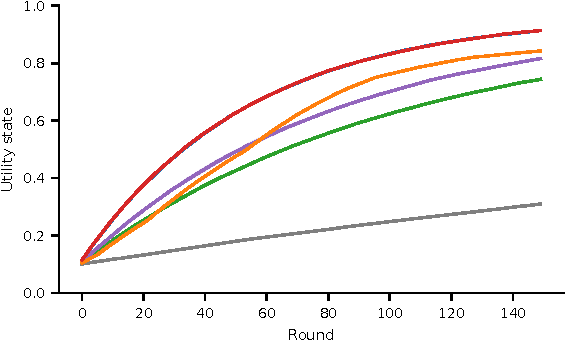
\includegraphics[width=\columnwidth]{fig_sim_accuracy_a.pdf}\label{fig:sima}}\\[2pt]%
\subfloat[Stress deadline (0.1 s)]{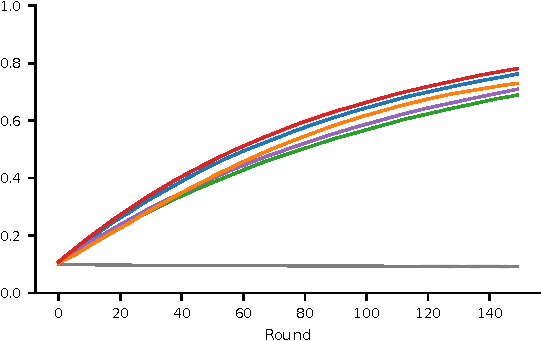
\includegraphics[width=\columnwidth]{fig_sim_accuracy_b.pdf}\label{fig:simb}}
\caption{Scheduler simulation utility-state trajectories (mean over five seeds). (a)~Nominal 2.0\,s deadline, where FedRAS matches fixed rank 16. (b)~0.1\,s deadline, where FedRAS downshifting separates from fixed rank 16.}
\label{fig:sim}
\end{figure}
\begin{figure}[pos=!ht]
\centering

\includegraphics[width=\columnwidth]{fig_sim_regimes_legend.pdf}\\[3pt]%
\subfloat[timely-delivery ratio]{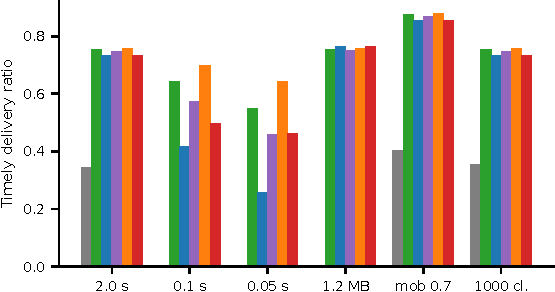
\includegraphics[width=\columnwidth]{fig_sim_regimes_a.pdf}\label{fig:simrega}}\\[2pt]%
\subfloat[bytes per round (MB)]{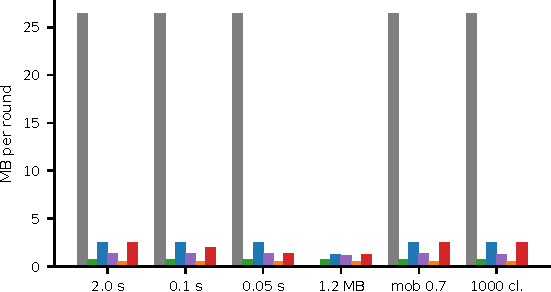
\includegraphics[width=\columnwidth]{fig_sim_regimes_b.pdf}\label{fig:simregb}}
\caption{Timely-delivery ratio and attempted bytes per method across simulator regimes, including the 1000-client scalability regime (five-seed means, final round). Full-model updates deliver nothing under stress and cannot be admitted at all under the binding budget.}
\label{fig:simreg}
\end{figure}
\begin{figure}[pos=!ht]
\centering

\includegraphics[width=\columnwidth]{fig_dp_study_legend.pdf}\\[3pt]%
\subfloat[objective loss vs.\ DP]{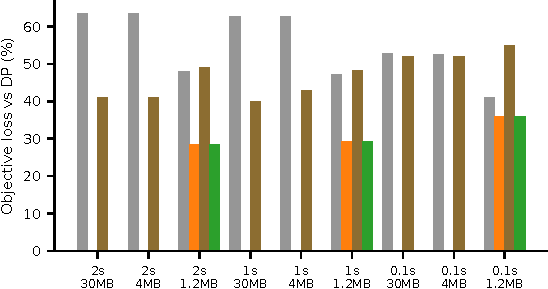
\includegraphics[width=\columnwidth]{fig_dp_study_a.pdf}\label{fig:dpa}}\\[2pt]%
\subfloat[DP runtime]{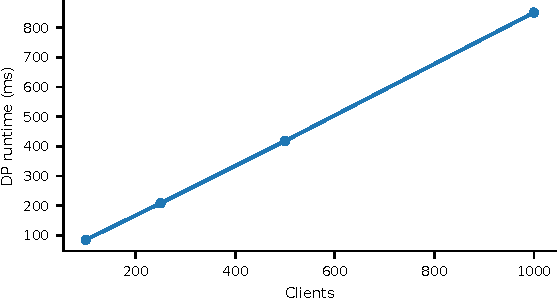
\includegraphics[width=\columnwidth]{fig_dp_study_b.pdf}\label{fig:dpb}}
\caption{Solver study. (a)~Objective loss of the heuristics relative to the DP across deadline and budget cells. (b)~DP runtime scaling with the client population.}
\label{fig:dp}
\end{figure}

\textbf{Sensitivity sweeps.} \cref{fig:sens} sweeps the provisioned width $r_{\max}$, the cohort size, and the label heterogeneity $\alpha$ on CIFAR-10 with FedRAS (five seeds per variant; the nominal reference uses ten seeds). Accuracy is flat in $r_{\max}$ and in the cohort size. Extreme label heterogeneity ($\alpha = 0.1$) reveals a second-order effect: rank-16 updates lose 0.32 percentage points relative to rank 4, consistent with capacity-amplified client drift, and full-model updates lose the most; FedRAS follows the rank-16 trajectory here, so a heterogeneity-aware downshift is a natural extension. The dominant effect of all three axes is on bytes and delivered updates (red, right axis of \cref{fig:sens}).

\textbf{Capacity-exponent sensitivity.} The half exponent of \cref{eq:cap} is a modeling choice anchored in the measured norms, so a solver-side sweep asks how the conclusions depend on it. Replacing $\sqrt{r/r_{\max}}$ with $(r/r_{\max})^{\gamma}$ for $\gamma\in\{0.25,0.5,0.75,1\}$ and re-solving 500-client instances (five seeds per cell) at the binding 1.2\,MB budget leaves every qualitative conclusion intact: value greedy loses 7--47\% of the objective (least at $\gamma=1$, where utilities linearize and value ordering packs well), value-per-byte greedy loses 0--43\%, and the budget-feasible fixed-rank-16 rule loses 8--48\%, while the DP's chosen mean rank stays within $7.5$--$8$ across all exponents, the downshifting direction does not depend on the exponent. Exactness earns its cost under every sub-linear capacity law, and the measured norm curve supports precisely the sub-linear regime.
\par
\begin{figure*}[pos=tbp]
\centering
\subfloat[Provisioned width $r_{\max}$]{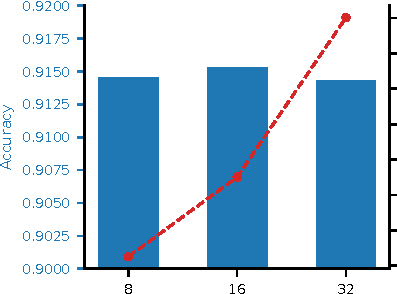
\includegraphics[width=.3548\linewidth]{fig_sensitivity_a.pdf}\label{fig:sensa}}\hfill%
\subfloat[Cohort size $K$]{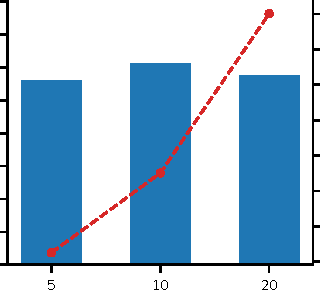
\includegraphics[width=.2858\linewidth]{fig_sensitivity_b.pdf}\label{fig:sensb}}\hfill%
\subfloat[Dirichlet $\alpha$]{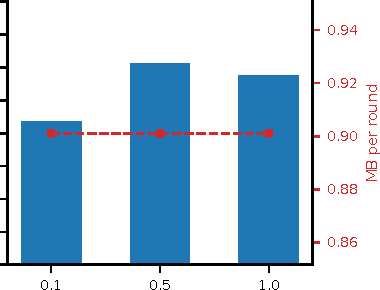
\includegraphics[width=.3392\linewidth]{fig_sensitivity_c.pdf}\label{fig:sensc}}
\caption{Sensitivity of the trainer to provisioned adapter width, cohort size, and label heterogeneity on CIFAR-10 with FedRAS (five seeds per variant; the nominal reference column uses ten seeds). Accuracy is flat in $r_{\max}$ and cohort size, with a second-order drop only at $\alpha = 0.1$; the dominant effect of all three axes is on bytes and delivered updates (red, right axis).}
\label{fig:sens}
\end{figure*}
\subsection{Efficiency and Robustness}
\label{sec:eff}
The final stage asks whether the architecture is deployable: what its scheduling and local computation cost, how it behaves under heterogeneous link classes and correlated data skew, under a structurally mismatched channel, under predictor error, and across datasets and stress axes.
\par
\textbf{Measured computation cost.} The measured local-training wall time is about 2.1\,s per client epoch on the reference GPU under evaluation-time sharing, two orders of magnitude above the 0.1\,s stress deadline, confirming that $\tau$ is the uplink delivery window rather than the round duration; the scheduling costs are reported with the solver study (\cref{sec:scale}).
\par
\textbf{Extended stress matrix.} \cref{tab:extended} extends the study along the delivery-side axes. Mobility-only scenarios leave all LoRA policies at parity at the nominal deadline with delivered ranks unchanged. By the closed form \cref{eq:rstar}, the per-client rank depends on rate and deadline alone, so no mobility law can force downshifting; mobility acts on admission, not on rank. The default Beta$(2,5)$, a milder Beta$(0.7,5)$, and a harsher Beta$(2,1)$ with $2.3\times$ the mean hazard all agree: under Beta$(2,1)$ the delivered rank stays pinned at 16 for every policy and accuracy stays at parity (0.9153/0.9156/0.9153 for rank 16/rank 4/FedRAS), while the timely-delivery ratio falls from 0.73 to 0.51. Mobility taxes delivery, never the rank choice, exactly as \cref{eq:rstar} predicts.
\par
Loosening the deadline to 10\,s restores full-model timely delivery to 0.52 without changing any LoRA accuracy.
\par
\begin{table}[pos=tbp]
\centering
\rmfamily
\small
\caption{Extended stress matrix of the real trainer (round-40 accuracy, five seeds). The mobility-only and $\alpha = 1.0$ scenarios probe extreme conditions; the last rows repeat the 0.1\,s deadline on CIFAR-100 and MNIST.}
\label{tab:extended}
\begin{tblr}
{
columns={co=-1},
cells={valign=m,halign=c},
columns={colsep=2pt},
rows={rowsep=2pt},
rows={ht=0pt},
stretch=0,
hline{1,Z}={wd=.08em},
hline{2}={wd=.05em},
cells={font=\fontsize{9pt}{9pt}},
row{1}={font=\bfseries\boldmath\fontsize{9pt}{9pt}},
row{even[2]}={bg=gray9!35},
}
Scenario & FedAvg & $r = 4$ & $r = 16$ & Random & FedRAS \\
deadline 10\,s & 0.9134 & 0.9144 & 0.9145 & 0.9141 & 0.9143 \\
mobility (milder) & 0.9115 & 0.9143 & 0.9141 & 0.9145 & 0.9141 \\
$\alpha = 0.1$ & 0.9022 & 0.9139 & 0.9107 & 0.9130 & 0.9109 \\
$\alpha = 1.0$ & 0.9142 & 0.9143 & 0.9144 & 0.9141 & 0.9144 \\
\end{tblr}
\end{table}

\textbf{Link-class heterogeneity and selection bias.} \textbf{SAGIN link profile.} Grouping the 20 clients into the ground, aerial, and satellite classes of a SAGIN, each with distinct rate and mobility laws, reproduces the aggregate parity at the nominal deadline while exposing the expected per-class structure: timely delivery is 0.84 for ground, 0.75 for aerial, and 0.64 for satellite clients (terminal-window means, five seeds). At this deadline the scheduler holds rank 16 across all classes, so the class gap reflects the link laws alone rather than rank allocation. The profile shows that the scheduler responds sensibly to client-class heterogeneity. Under the 0.1\,s deadline the downshifting is per class and it is precisely what protects the weakest class: FedRAS delivers a timely-delivery ratio of $0.51$ in aggregate ($0.57$ for ground, $0.42$ for aerial, and $0.43$ for satellite clients) with a delivered rank of $13.1$, beating fixed rank 16 ($0.44$ timely) at $22\%$ fewer bytes. Against the same fixed width, whose per-class timely ratios are 0.54 (ground), 0.32 (aerial), and 0.19 (satellite), the scheduler more than doubles the satellite class's timely delivery while the ground class---held at the full width---loses nothing: the class gap that the link laws impose on a fixed payload is largely closed by letting the rank move with the link.
\par
\textbf{Correlated link--data skew.} Correlating this class structure with the data sharpens the question: when the weak-link classes live exclusively on the aerial and satellite clients, the participation bias that no aggregation rule can remove is measurable but bounded. At the 0.1\,s deadline the weak-link half of the classes trails the strong-link half by 4.9 points under FedRAS, against 5.8 under fixed rank 16 and 3.2 under fixed rank 4; FedRAS sits within a point and a half of the low-rank fairness floor while holding three times its delivered capacity, and its aggregate accuracy (0.9125) stays within the equivalence band. The bias is a property of link-dependent participation, not of the rank rule; charging it fully is what per-client fairness accounting would require, and it composes with the scheduler as an additional constraint rather than a redesign.
\par
\textbf{De-circularized delivery arm.} The headline evaluation generates realized delivery from the same hazard model the scheduler optimizes, with oracle link states. To test that the delivered-capacity gains are not an artifact of this closed loop, a dedicated arm replaces both. Realized rates follow a per-client first-order autoregressive (AR(1)) log-process with autocorrelation $0.6$ and stationary marginal equal to the headline LogNormal$(2.5, 0.7)$ law, so the history-based estimate, an exponential moving average (EMA) with coefficient $0.5$ over past realized rates, exactly the estimation step of \cref{alg:fedras}, is stale. Realized delivery is structural: a propagation delay of $5$\,ms, a handover event with probability $0.15$ adding $20$\,ms, and a loss event with probability $1 - e^{-1.5\mu_i^t}$, rather than a draw from the hazard model. The arm runs at the $0.1$\,s stress deadline. The scheduler plans against the stale EMA estimate and the mobility intensity alone; delivery succeeds iff the structural delivery time (propagation, handover, and transmission at the realized rate) meets the deadline and no loss event occurs.
\par
\textbf{Results.} Under the structural channel the ordering of the hazard-model arm survives with stale, noisy estimates: FedRAS delivers a timely-delivery ratio of 0.59 at 0.73\,MB with delivered rank 13.1, against 0.52 at 0.90\,MB for fixed rank 16, the capacity-matched comparator, while the fixed low rank keeps the timely lead (0.67 at 0.23\,MB) at a third of the delivered capacity, and full-model updates deliver nothing. Accuracy stays at parity (0.915--0.916) throughout, as expected with the strong backbone. The delivered-capacity gains therefore survive a structurally mismatched channel in both direction and mechanism---buying delivery where it is cheap by shedding rank and preserving capacity where it pays---and the magnitudes soften relative to the oracle arm, which is the honest price of the closed-loop assumption the headline tiers carry.
\par
\textbf{Delivery-predictor sensitivity.} \par
\begin{figure*}[pos=tbp]
\centering
\subfloat[reliability at the 0.1\,s deadline]{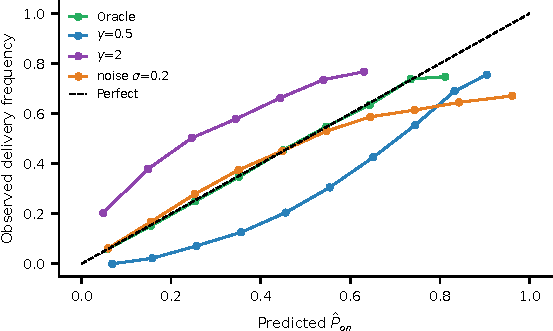
\includegraphics[width=.49\linewidth]{fig_calibration_a.pdf}\label{fig:caliba}}\hfill%
\subfloat[objective loss under true probabilities]{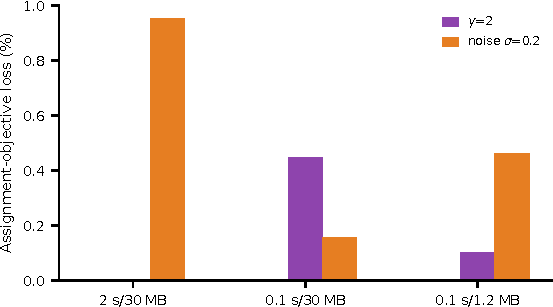
\includegraphics[width=.49\linewidth]{fig_calibration_b.pdf}\label{fig:calibb}}
\caption{Delivery-predictor calibration study (500 clients, 150 round-instances per cell). (a)~Reliability at the 0.1\,s deadline; with oracle link state the hazard predictor is calibrated by construction, while the power-distorted ($\gamma$) and noisy variants are measurably miscalibrated. (b)~Assignment-objective loss of optimizing against the distorted predictor, evaluated under true probabilities, at most 1\% on average in every cell; the $\gamma = 0.5$ loss is $<0.001\%$ throughout, labeled explicitly on the log-scaled panel.}
\label{fig:calib}
\end{figure*}
\par
The calibration study of \cref{fig:calib} measures both the fidelity of the deployed predictor and the scheduling cost of its errors (500 clients). With the oracle link state of the setup, the hazard predictor \cref{eq:hazard} is calibrated by construction. Deliberately distorted variants, power distortions of the predicted probability and multiplicative lognormal noise, are measurably miscalibrated, yet the resulting assignment-objective loss, evaluated under the true probabilities, stays below 1\% on average in every cell. The loss follows the structure of the error: power distortions cost most under the stress deadline, where rank ordering matters most, while noise costs most in the nominal slack cell, where it perturbs an otherwise near-uniform rank preference. Mis-prediction therefore degrades the objective smoothly rather than catastrophically, and the observed delivery outcomes of \cref{alg:fedras} are exactly the signal from which a per-client predictor would be recalibrated.
\par

\par
\subsection{Scale and Solver Study}
\label{sec:scale}
The simulation tier asks whether the trainer conclusions survive an order of magnitude more clients, and the solver study asks what exactness costs and returns at that scale.
\par
\textbf{Scheduler simulation across regimes.} \label{sec:simsim}
\cref{tab:scalemain}(a) summarizes the simulator across regimes at the final round. In the nominal regime, FedRAS matches fixed rank 16 and dominates every low-rank policy. Under the 0.1\,s deadline, FedRAS leads fixed rank 16 at 20\% fewer bytes (2.0 versus 2.5\,MB), and full-model updates deliver nothing. Under the binding 1.2\,MB budget, full-model updates cannot be admitted even once, while FedRAS and rank 16 tie. The mobility-stress and 1000-client regimes show the same pattern: FedRAS and fixed rank 16 coincide at the top of the utility column, so scheduling separates only where deadlines or budgets bind. A final cell repeats the stylized protocol of the earlier literature: with the $s(r)$ payload model the ordering is preserved, confirming that the conclusions are not an artifact of the payload accounting.
\par
\textbf{Where the simulator gain comes from.} Fixed rank 16 spends uniformly, weak-link clients miss deadlines while strong-link clients are under-served, whereas FedRAS reallocates, holding high ranks where delivery survives them and downshifting or skipping the rest. Reliability-only optimization fails the other way, buying timely delivery with capacity. The dynamic program between these extremes prices capacity and delivery in a common unit, and the grid makes the resulting knapsack exactly solvable.
\par
\textbf{Trajectories.} \cref{fig:sim} shows the nominal and 0.1\,s trajectories, and \cref{fig:simreg} the delivery-side view across regimes.
\par
\label{sec:dp_study}
\textbf{Solver study: heuristic gaps and runtime.} \cref{tab:scalemain}(b) reports the scheduling study with the identical ceiling discretization for the DP and every heuristic. When the byte budget is slack, value greedy and the fixed rank-16 rule are already optimal, so the choice of scheduler matters little; the value-per-byte greedy, by contrast, collapses to a smallest-rank preference and already loses up to 63.6\% of the objective in the slack cells. The interesting regimes are the binding ones: once the budget binds, every heuristic loses a substantial fraction of the objective, up to 54.8\% for the cohort-myopic rule, while the DP reaches the optimum of the discretized single-round estimated problem in every cell. Its runtime is sub-second at 500 clients and scales linearly to 1000 (\cref{fig:dp}); scheduling precedes the uplink window and is charged to round setup rather than $\tau$ ($23$--$421$\,ms per round for the DP across the evaluated grid widths; sub-millisecond decisions for the per-client rule).
\par
\textbf{Why the heuristics fail where they do.} The failure modes are structural rather than numerical, and both were already visible in the models. Value-per-byte pricing divides a capacity gain that saturates with rank by a payload that grows linearly in \cref{eq:size}, so its ratio favors the smallest rank regardless of link state. Fixed rank 16 and value greedy fail only under scarcity, where choosing which candidates to drop is precisely the admission coupling that per-client rules cannot resolve. The DP runtime grows with the client count but is far more sensitive to the budget grid width, which is why it is fastest under exactly the binding budgets that need it most.
\par
\textbf{Grid sweep.} A dedicated grid sweep around the default step bounds the quantization error at about 3\% in the binding regime and below 1\% in slack regimes; a finer step reduces it further at a known runtime cost. The grid exactness claim therefore applies to a grid whose quantization error is bounded, measured, and adjustable.


\label{sec:rob}
\section{Discussion and Limitations}
\label{sec:discussion}
\subsection{Interpretation and Deployment}
\textbf{Why the strong backbone licenses network control of the rank.} With a strong frozen backbone, transmitted rank does not measurably change test accuracy. This invariance is the enabling condition of the architecture rather than a weakness of the results: precisely because accuracy does not depend on the rank, the rank is free to be set by the link, and the scheduler's advantage appears as delivered adaptation capacity, bytes, and energy rather than as accuracy points---the contribution currency of communication-efficiency and client-selection systems, here evaluated at non-degraded accuracy. When the backbone is weak enough to need adaptation, the preserved capacity converts into accuracy along the measured backbone-quality sweep. When the pool fits the cap and the budget accommodates every candidate at $r_{\max}$, the per-client rule is already optimal (\cref{prop:cohort}) at zero overhead, and exact scheduling pays only when the budget binds or the pool must be culled. Under extreme label heterogeneity high ranks lose accuracy through capacity-amplified drift, and under tight deadlines the weakest client class still delivers least.
\par
\textbf{Deployment.} Calibrate the deadline ladder from the real payload of the widest rank, size the byte budget at ten times the grid cost of $r_{\max}$, use \cref{prop:cohort} as a runtime switch, and treat the predictor as a monitored plug-in, since distortions cost at most about $1\%$ of the objective (\cref{fig:calib}). The delivered-capacity advantage translates directly into operator currencies: under the airtime-proportional transmit-energy model, the stress configuration delivers about $41\%$ more adaptation capacity per joule than fixed rank 16, whose airtime is $59\%$ spent on updates that never arrive, and matching FedRAS's timely ratio would require about $1.5\times$ the uplink rate for the fixed-rank fleet. FedRAS is an aggregator-side module that leaves client training untouched.
\par
\subsection{Limitations}
The results are gains in delivered adaptation capacity in the evaluated setting and, where the backbone needs adaptation, in accuracy---not universal accuracy gains---and centralized pretraining is a standing premise of parameter-efficient FL. The hazard model \cref{eq:hazard} assumes the closed-form realization with oracle link states, which the de-circularized arm probes but does not remove, and rates are drawn independently, so the shared-spectrum case is untested. The $\sqrt{r}$ capacity law assumes the delivered-update norm is a faithful proxy for contribution, an assumption the exponent sweep bounds. Conclusions are horizon-bound to forty rounds on a star topology, and the CNN covariate-shift tier marks a task boundary where adapters preserve rather than recover accuracy. This work proposes no protection mechanism and makes no privacy claim, and differential-privacy accounting, secure aggregation, and Byzantine robustness compose orthogonally with rank scheduling \cite{bonawitz2017secureagg,wei2023pfl_dp}.
\par
\subsection{Future Work}
The immediate extensions are horizon-aware scheduling that carries budgets across rounds and exploits mobility correlation, per-client predictors calibrated on measured wireless traces, the correlated-spectrum case where clients share a cell or beam, heterogeneity-aware capacity terms, and composition with privacy accounting. Transformer backbones beyond the tiny ViT tier, wider rank sets, and validation on operational mobile-edge networks would further test where rank scheduling pays.
\par
\section{Conclusion}
\label{sec:conclusion}
FedRAS treats the LoRA rank as a schedulable network resource accounted at its real serialized size and runs a closed round loop in which client--rank pairs are priced by the payload-conditioned hazard model and a saturating capacity gain, admission and rank are decided jointly by an exact grid dynamic program with a provably optimal cheap fallback, and heterogeneous-rank updates are merged by frozen-factor masked averaging. The formulation yields the closed form $r_i^\star=\bar R_i^t\tau/(16c)$ and a one-pass check that invokes exact solving only where scarcity couples decisions.
\par
In the single currency of delivered update mass, FedRAS delivers the most of any evaluated policy under the $0.1$\,s stress deadline---$22\%$ more timely updates than the capacity-matched fixed rank 16 at $23\%$ fewer bytes and $42\%$ more update mass than the timely-count leader fixed rank 4 (ten of ten paired seeds, $p=0.002$)---at statistically equivalent accuracy, while full-model updates miss every stress deadline and the loop delivers nothing. A six-point backbone-quality sweep locates the conversion boundary: delivered capacity turns into accuracy once the backbone falls below roughly $0.8$, reaching $+1.1$ points over link-oblivious schedules at backbone accuracy $0.53$, one point under covariate shift on the transformer tier, and three points over the zero-communication control with disjoint pretraining. Under a binding $0.4$\,MB budget the dynamic program beats the strongest value greedy by twelve timely points at fewer bytes, and every link-aware rule, including re-implementations after ROBA/TSFA and FedARA, beats the link-oblivious schedules on the weak-backbone task.
\par
The gains come from the pricing rather than the solver's arithmetic, and exactness is free in slack regimes through the runtime switch and decisive where budgets bind. The open bounds are the independent-generation assumption on link laws, the bounded capacity exponent, the covariate-shift boundary, and the forty-round horizon. The next steps are horizon-aware scheduling, trace-calibrated predictors, correlated spectrum, and deployment validation, all governed by the condition FedRAS established, that the delivery probability of the payload, not the expectation of its delay, should set the rank.
\par
\section*{CRediT authorship contribution statement}
\textbf{Wenyu Ma:} Methodology, Software, Validation, Investigation, Formal analysis, Data curation, Visualization, Writing -- original draft.
\textbf{Xinlei Liu:} Conceptualization, Funding acquisition, Resources, Project administration, Supervision, Writing -- review \& editing.
\textbf{Tao Hu:} Conceptualization, Funding acquisition, Resources, Project administration, Supervision, Writing -- review \& editing.
\section*{Declaration of competing interest}
The authors declare that they have no known competing financial interests or personal relationships that could have appeared to influence the work reported in this paper.
\section*{Funding}
This work was supported in part by the National Key Research and Development Program of China (No.\ 2024YFB2907201, No.\ 2024YFB2907202).
\section*{Declaration of generative AI and AI-assisted technologies in the manuscript preparation process}
During the preparation of this work the authors used GLM-5.3 in order to improve the language and readability of the manuscript. After using this tool, the authors reviewed and edited the content as needed and take full responsibility for the content of the published article.
\section*{Data availability}
The complete source code (trainer, simulator, solver, and analysis scripts) and the result data backing every table and figure, per-run configuration files, per-seed result tables, and raw training logs, are publicly available at \url{https://github.com/Jude-max11/FedRAS}.
\bibliographystyle{elsarticle-num}
\bibliography{reference}
\end{document}
